\documentclass[a4paper]{book}
\usepackage{a4wide}
\usepackage{makeidx}
\usepackage{graphicx}
\usepackage{multicol}
\usepackage{float}
\usepackage{listings}
\usepackage{color}
\usepackage{textcomp}
\usepackage{alltt}
\usepackage{times}
\usepackage{ifpdf}
\ifpdf
\usepackage[pdftex,
            pagebackref=true,
            colorlinks=true,
            linkcolor=blue,
            unicode
           ]{hyperref}
\else
\usepackage[ps2pdf,
            pagebackref=true,
            colorlinks=true,
            linkcolor=blue,
            unicode
           ]{hyperref}
\usepackage{pspicture}
\fi
\usepackage[utf8]{inputenc}
\usepackage{doxygen}
\lstset{language=C++,inputencoding=utf8,basicstyle=\footnotesize,breaklines=true,breakatwhitespace=true,tabsize=8,numbers=left }
\makeindex
\setcounter{tocdepth}{3}
\renewcommand{\footrulewidth}{0.4pt}
\begin{document}
\hypersetup{pageanchor=false}
\begin{titlepage}
\vspace*{7cm}
\begin{center}
{\Large Procedural Game Plot Generation Prototype }\\
\vspace*{1cm}
{\large Generated by Doxygen 1.6.3}\\
\vspace*{0.5cm}
{\small Sat Jul 24 16:03:36 2010}\\
\end{center}
\end{titlepage}
\clearemptydoublepage
\pagenumbering{roman}
\tableofcontents
\clearemptydoublepage
\pagenumbering{arabic}
\hypersetup{pageanchor=true}
\chapter{Class Index}
\section{Class Hierarchy}
This inheritance list is sorted roughly, but not completely, alphabetically:\begin{DoxyCompactList}
\item \contentsline{section}{Application}{\pageref{classApplication}}{}
\item \contentsline{section}{Decision}{\pageref{classDecision}}{}
\item \contentsline{section}{Decisions}{\pageref{classDecisions}}{}
\item \contentsline{section}{DiscreteRange}{\pageref{classDiscreteRange}}{}
\item \contentsline{section}{GameObject}{\pageref{classGameObject}}{}
\begin{DoxyCompactList}
\item \contentsline{section}{MoveableGameObject}{\pageref{classMoveableGameObject}}{}
\item \contentsline{section}{PlayerCharacter}{\pageref{classPlayerCharacter}}{}
\end{DoxyCompactList}
\item \contentsline{section}{IsometricConversions}{\pageref{classIsometricConversions}}{}
\item \contentsline{section}{Option}{\pageref{classOption}}{}
\item \contentsline{section}{Options}{\pageref{classOptions}}{}
\item \contentsline{section}{Overlay}{\pageref{classOverlay}}{}
\begin{DoxyCompactList}
\item \contentsline{section}{IsometricGrid}{\pageref{classIsometricGrid}}{}
\end{DoxyCompactList}
\item \contentsline{section}{Plot}{\pageref{classPlot}}{}
\item \contentsline{section}{Program}{\pageref{classProgram}}{}
\item \contentsline{section}{RandomGenerator}{\pageref{classRandomGenerator}}{}
\item \contentsline{section}{Result}{\pageref{classResult}}{}
\item \contentsline{section}{World}{\pageref{classWorld}}{}
\end{DoxyCompactList}

\chapter{Class Index}
\section{Class List}
Here are the classes, structs, unions and interfaces with brief descriptions:\begin{DoxyCompactList}
\item\contentsline{section}{\hyperlink{classApplication}{Application} }{\pageref{classApplication}}{}
\item\contentsline{section}{\hyperlink{classDecision}{Decision} }{\pageref{classDecision}}{}
\item\contentsline{section}{\hyperlink{classDecisions}{Decisions} }{\pageref{classDecisions}}{}
\item\contentsline{section}{\hyperlink{classDiscreteRange}{DiscreteRange} }{\pageref{classDiscreteRange}}{}
\item\contentsline{section}{\hyperlink{classGameObject}{GameObject} }{\pageref{classGameObject}}{}
\item\contentsline{section}{\hyperlink{classIsometricConversions}{IsometricConversions} }{\pageref{classIsometricConversions}}{}
\item\contentsline{section}{\hyperlink{classIsometricGrid}{IsometricGrid} }{\pageref{classIsometricGrid}}{}
\item\contentsline{section}{\hyperlink{classMoveableGameObject}{MoveableGameObject} }{\pageref{classMoveableGameObject}}{}
\item\contentsline{section}{\hyperlink{classOption}{Option} }{\pageref{classOption}}{}
\item\contentsline{section}{\hyperlink{classOptions}{Options} }{\pageref{classOptions}}{}
\item\contentsline{section}{\hyperlink{classOverlay}{Overlay} }{\pageref{classOverlay}}{}
\item\contentsline{section}{\hyperlink{classPlayerCharacter}{PlayerCharacter} }{\pageref{classPlayerCharacter}}{}
\item\contentsline{section}{\hyperlink{classPlot}{Plot} }{\pageref{classPlot}}{}
\item\contentsline{section}{\hyperlink{classProgram}{Program} }{\pageref{classProgram}}{}
\item\contentsline{section}{\hyperlink{classRandomGenerator}{RandomGenerator} }{\pageref{classRandomGenerator}}{}
\item\contentsline{section}{\hyperlink{classResult}{Result} }{\pageref{classResult}}{}
\item\contentsline{section}{\hyperlink{classWorld}{World} }{\pageref{classWorld}}{}
\end{DoxyCompactList}

\chapter{File Index}
\section{File List}
Here is a list of all documented files with brief descriptions:\begin{DoxyCompactList}
\item\contentsline{section}{source/{\bfseries Application.h} }{\pageref{Application_8h}}{}
\item\contentsline{section}{source/\hyperlink{ApplicationModule_8cpp}{ApplicationModule.cpp} }{\pageref{ApplicationModule_8cpp}}{}
\item\contentsline{section}{source/\hyperlink{ApplicationModule_8h}{ApplicationModule.h} }{\pageref{ApplicationModule_8h}}{}
\item\contentsline{section}{source/\hyperlink{ApplicationModuleExitCode_8h}{ApplicationModuleExitCode.h} }{\pageref{ApplicationModuleExitCode_8h}}{}
\item\contentsline{section}{source/bbn/{\bfseries BBN\_\-Decision.h} }{\pageref{BBN__Decision_8h}}{}
\item\contentsline{section}{source/bbn/\hyperlink{BBN__Exception_8cpp}{BBN\_\-Exception.cpp} }{\pageref{BBN__Exception_8cpp}}{}
\item\contentsline{section}{source/bbn/\hyperlink{BBN__Exception_8h}{BBN\_\-Exception.h} }{\pageref{BBN__Exception_8h}}{}
\item\contentsline{section}{source/bbn/{\bfseries BBN\_\-Given.h} }{\pageref{BBN__Given_8h}}{}
\item\contentsline{section}{source/bbn/{\bfseries BBN\_\-Info.h} }{\pageref{BBN__Info_8h}}{}
\item\contentsline{section}{source/bbn/{\bfseries BBN\_\-Option.h} }{\pageref{BBN__Option_8h}}{}
\item\contentsline{section}{source/bbn/{\bfseries BBN\_\-Plot.h} }{\pageref{BBN__Plot_8h}}{}
\item\contentsline{section}{source/bbn/{\bfseries BBN\_\-Prob.h} }{\pageref{BBN__Prob_8h}}{}
\item\contentsline{section}{source/bbn/{\bfseries BBN\_\-Random.h} }{\pageref{BBN__Random_8h}}{}
\item\contentsline{section}{source/game/\hyperlink{AccessibleArea_8cpp}{AccessibleArea.cpp} }{\pageref{AccessibleArea_8cpp}}{}
\item\contentsline{section}{source/game/\hyperlink{AccessibleArea_8h}{AccessibleArea.h} }{\pageref{AccessibleArea_8h}}{}
\item\contentsline{section}{source/game/\hyperlink{GameObject_8cpp}{GameObject.cpp} }{\pageref{GameObject_8cpp}}{}
\item\contentsline{section}{source/game/\hyperlink{GameObject_8h}{GameObject.h} }{\pageref{GameObject_8h}}{}
\item\contentsline{section}{source/game/\hyperlink{IsometricGrid_8cpp}{IsometricGrid.cpp} }{\pageref{IsometricGrid_8cpp}}{}
\item\contentsline{section}{source/game/\hyperlink{IsometricGrid_8h}{IsometricGrid.h} }{\pageref{IsometricGrid_8h}}{}
\item\contentsline{section}{source/game/\hyperlink{MoveableGameObject_8cpp}{MoveableGameObject.cpp} }{\pageref{MoveableGameObject_8cpp}}{}
\item\contentsline{section}{source/game/\hyperlink{MoveableGameObject_8h}{MoveableGameObject.h} }{\pageref{MoveableGameObject_8h}}{}
\item\contentsline{section}{source/game/\hyperlink{Overlay_8cpp}{Overlay.cpp} }{\pageref{Overlay_8cpp}}{}
\item\contentsline{section}{source/game/\hyperlink{Overlay_8h}{Overlay.h} }{\pageref{Overlay_8h}}{}
\item\contentsline{section}{source/game/\hyperlink{Room_8cpp}{Room.cpp} }{\pageref{Room_8cpp}}{}
\item\contentsline{section}{source/game/\hyperlink{Room_8h}{Room.h} }{\pageref{Room_8h}}{}
\item\contentsline{section}{source/game/\hyperlink{Scene_8cpp}{Scene.cpp} }{\pageref{Scene_8cpp}}{}
\item\contentsline{section}{source/game/\hyperlink{Scene_8h}{Scene.h} }{\pageref{Scene_8h}}{}
\item\contentsline{section}{source/game/\hyperlink{Viewport_8cpp}{Viewport.cpp} }{\pageref{Viewport_8cpp}}{}
\item\contentsline{section}{source/game/\hyperlink{Viewport_8h}{Viewport.h} }{\pageref{Viewport_8h}}{}
\item\contentsline{section}{source/game/\hyperlink{World_8cpp}{World.cpp} }{\pageref{World_8cpp}}{}
\item\contentsline{section}{source/game/\hyperlink{World_8h}{World.h} }{\pageref{World_8h}}{}
\item\contentsline{section}{source/game/game\_\-objects/{\bfseries HotelGroundFloor.h} }{\pageref{HotelGroundFloor_8h}}{}
\item\contentsline{section}{source/game/game\_\-objects/\hyperlink{PlayerCharacter_8cpp}{PlayerCharacter.cpp} }{\pageref{PlayerCharacter_8cpp}}{}
\item\contentsline{section}{source/game/game\_\-objects/\hyperlink{PlayerCharacter_8h}{PlayerCharacter.h} }{\pageref{PlayerCharacter_8h}}{}
\item\contentsline{section}{source/game/game\_\-objects/\hyperlink{Prop_8cpp}{Prop.cpp} }{\pageref{Prop_8cpp}}{}
\item\contentsline{section}{source/game/game\_\-objects/\hyperlink{Prop_8h}{Prop.h} }{\pageref{Prop_8h}}{}
\item\contentsline{section}{source/main\_\-menu/\hyperlink{MainMenu_8cpp}{MainMenu.cpp} }{\pageref{MainMenu_8cpp}}{}
\item\contentsline{section}{source/main\_\-menu/\hyperlink{MainMenu_8h}{MainMenu.h} }{\pageref{MainMenu_8h}}{}
\item\contentsline{section}{source/misc/\hyperlink{logging_8h}{logging.h} }{\pageref{logging_8h}}{}
\item\contentsline{section}{source/monster\_\-generator\_\-demo/{\bfseries Monster.h} }{\pageref{Monster_8h}}{}
\item\contentsline{section}{source/monster\_\-generator\_\-demo/{\bfseries MonsterGeneratorDemo.h} }{\pageref{MonsterGeneratorDemo_8h}}{}
\end{DoxyCompactList}

\chapter{Class Documentation}
\hypertarget{classAccessibleArea}{
\section{AccessibleArea Class Reference}
\label{classAccessibleArea}\index{AccessibleArea@{AccessibleArea}}
}


{\ttfamily \#include $<$AccessibleArea.h$>$}

Inheritance diagram for AccessibleArea:\begin{figure}[H]
\begin{center}
\leavevmode
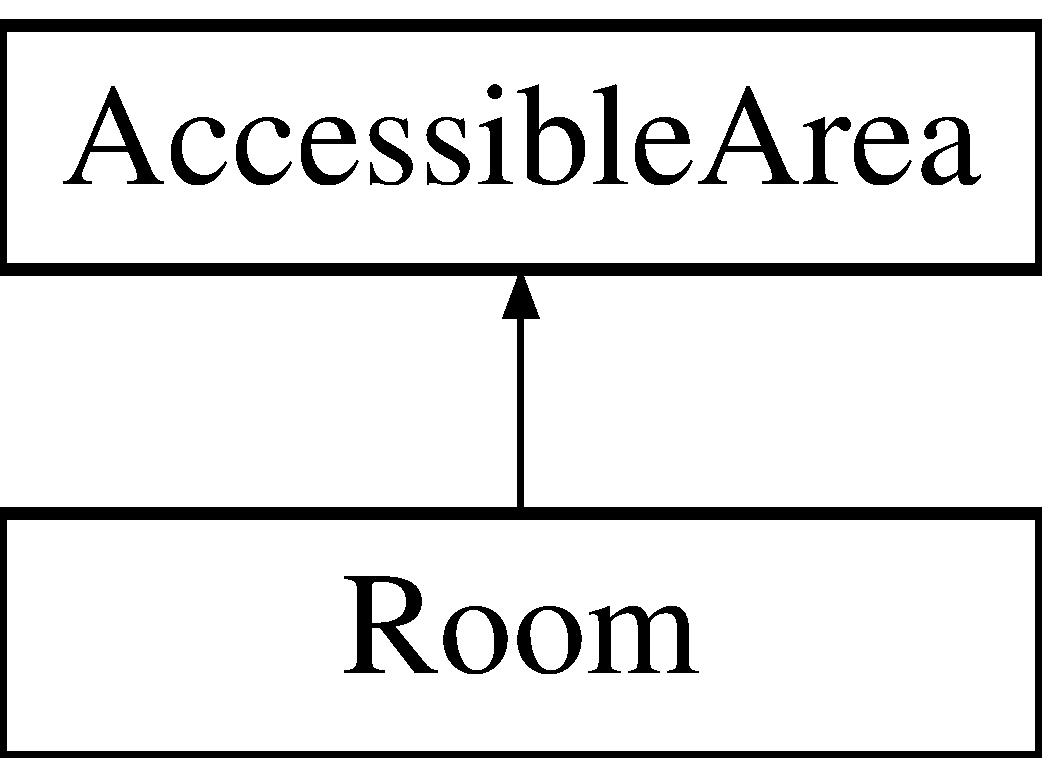
\includegraphics[height=2cm]{classAccessibleArea}
\end{center}
\end{figure}
\subsection*{Public Member Functions}
\begin{DoxyCompactItemize}
\item 
\hypertarget{classAccessibleArea_a2f00691133643b196a7f695c3d7f36be}{
{\bfseries AccessibleArea} (\hyperlink{classScene}{Scene} $\ast$, double, double, double, double)}
\label{classAccessibleArea_a2f00691133643b196a7f695c3d7f36be}

\item 
\hypertarget{classAccessibleArea_a77376ad943429e7acd10403ff70a4105}{
virtual void {\bfseries draw} (void)}
\label{classAccessibleArea_a77376ad943429e7acd10403ff70a4105}

\end{DoxyCompactItemize}
\subsection*{Protected Attributes}
\begin{DoxyCompactItemize}
\item 
\hypertarget{classAccessibleArea_a41e88a8d1e45ba68b18f09da81623417}{
\hyperlink{classScene}{Scene} $\ast$ {\bfseries scene}}
\label{classAccessibleArea_a41e88a8d1e45ba68b18f09da81623417}

\item 
\hypertarget{classAccessibleArea_ab73273146fc9a7f5b56014d6009dc9d8}{
std::list$<$ CL\_\-Pointd $>$ {\bfseries points}}
\label{classAccessibleArea_ab73273146fc9a7f5b56014d6009dc9d8}

\end{DoxyCompactItemize}


\subsection{Detailed Description}
Provides areas defined by a series of points and an area where the player's character may walk within, therefore provides rules for collisions. More specific implementations exist such as \hyperlink{classRoom}{Room}. 

The documentation for this class was generated from the following files:\begin{DoxyCompactItemize}
\item 
source/game/\hyperlink{AccessibleArea_8h}{AccessibleArea.h}\item 
source/game/\hyperlink{AccessibleArea_8cpp}{AccessibleArea.cpp}\end{DoxyCompactItemize}

\hypertarget{classApplication}{
\section{Application Class Reference}
\label{classApplication}\index{Application@{Application}}
}


{\ttfamily \#include $<$Application.h$>$}\subsection*{Public Member Functions}
\begin{DoxyCompactItemize}
\item 
\hypertarget{classApplication_abbda0eddef2dd5fcce957a82373ecb6c}{
virtual int {\bfseries main} (const std::vector$<$ CL\_\-String $>$ \&args)}
\label{classApplication_abbda0eddef2dd5fcce957a82373ecb6c}

\end{DoxyCompactItemize}
\subsection*{Static Public Member Functions}
\begin{DoxyCompactItemize}
\item 
static void \hyperlink{classApplication_a1112e5aede67cff7aad4c8fb4be3e3af}{log} (const int, const CL\_\-String \&)
\end{DoxyCompactItemize}


\subsection{Detailed Description}
The \hyperlink{classApplication}{Application} object provides transition between the modules of the overall application. It instantiates a clanLib window and instantiates the other shared parts of the engine. 

\subsection{Member Function Documentation}
\hypertarget{classApplication_a1112e5aede67cff7aad4c8fb4be3e3af}{
\index{Application@{Application}!log@{log}}
\index{log@{log}!Application@{Application}}
\subsubsection[{log}]{\setlength{\rightskip}{0pt plus 5cm}void Application::log (const int {\em level}, \/  const CL\_\-String \& {\em message})\hspace{0.3cm}{\ttfamily  \mbox{[}static\mbox{]}}}}
\label{classApplication_a1112e5aede67cff7aad4c8fb4be3e3af}
Outputs the message to the console and the active log file. 

The documentation for this class was generated from the following files:\begin{DoxyCompactItemize}
\item 
source/Application.h\item 
source/Application.cpp\end{DoxyCompactItemize}

\hypertarget{classApplicationModule}{
\section{ApplicationModule Class Reference}
\label{classApplicationModule}\index{ApplicationModule@{ApplicationModule}}
}


{\ttfamily \#include $<$ApplicationModule.h$>$}

Inheritance diagram for ApplicationModule:\begin{figure}[H]
\begin{center}
\leavevmode
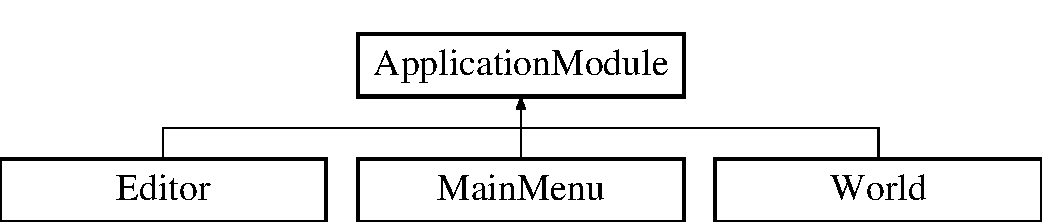
\includegraphics[height=2cm]{classApplicationModule}
\end{center}
\end{figure}
\subsection*{Public Member Functions}
\begin{DoxyCompactItemize}
\item 
\hyperlink{classApplicationModule_adee14a760314582348ee3205097fea4c}{ApplicationModule} (const CL\_\-DisplayWindow \&)
\item 
ApplicationModuleExitCode \hyperlink{classApplicationModule_a72494b92d2b093e0827893f527535a1f}{run} (void)
\item 
\hypertarget{classApplicationModule_a2c4555686e9bd25708a112ac852c3a17}{
CL\_\-GraphicContext $\ast$ {\bfseries get\_\-gc} (void)}
\label{classApplicationModule_a2c4555686e9bd25708a112ac852c3a17}

\item 
\hypertarget{classApplicationModule_a6c9168a94ebee4eacc23b7ce58878ce7}{
CL\_\-GUIManager $\ast$ {\bfseries get\_\-gui\_\-manager} (void)}
\label{classApplicationModule_a6c9168a94ebee4eacc23b7ce58878ce7}

\end{DoxyCompactItemize}
\subsection*{Protected Member Functions}
\begin{DoxyCompactItemize}
\item 
\hypertarget{classApplicationModule_a8976aad9f18518a03d83be61283d9b6e}{
virtual void {\bfseries draw} (void)}
\label{classApplicationModule_a8976aad9f18518a03d83be61283d9b6e}

\item 
\hypertarget{classApplicationModule_a1bfe895c2c5f3d14e32973db2ec51723}{
virtual void {\bfseries update} (void)}
\label{classApplicationModule_a1bfe895c2c5f3d14e32973db2ec51723}

\item 
\hypertarget{classApplicationModule_ac182827a21ffdafb13327e24c3aff773}{
virtual void {\bfseries wm\_\-repaint} (void)}
\label{classApplicationModule_ac182827a21ffdafb13327e24c3aff773}

\item 
void \hyperlink{classApplicationModule_a2fb74c01602d0a030eb7335543580be3}{draw\_\-loading} (void)
\item 
\hypertarget{classApplicationModule_ad21cf0501238dd52bbe4c84606f6cb91}{
virtual void {\bfseries on\_\-window\_\-close} (void)}
\label{classApplicationModule_ad21cf0501238dd52bbe4c84606f6cb91}

\item 
\hypertarget{classApplicationModule_aec7e75cf19261da574bc0f238b430738}{
virtual void {\bfseries on\_\-key\_\-down} (const CL\_\-InputEvent \&key, const CL\_\-InputState \&state)}
\label{classApplicationModule_aec7e75cf19261da574bc0f238b430738}

\item 
\hypertarget{classApplicationModule_acbff2a3dc36d72449a47ac0bb139719b}{
virtual void {\bfseries on\_\-key\_\-up} (const CL\_\-InputEvent \&key, const CL\_\-InputState \&state)}
\label{classApplicationModule_acbff2a3dc36d72449a47ac0bb139719b}

\item 
\hypertarget{classApplicationModule_a59c95ac03dc85010f132d5bbb628a481}{
virtual void {\bfseries on\_\-mouse\_\-down} (const CL\_\-InputEvent \&key, const CL\_\-InputState \&state)}
\label{classApplicationModule_a59c95ac03dc85010f132d5bbb628a481}

\item 
\hypertarget{classApplicationModule_a1017f6c73e46f9e2167ad71960bece8d}{
virtual void {\bfseries on\_\-mouse\_\-up} (const CL\_\-InputEvent \&key, const CL\_\-InputState \&state)}
\label{classApplicationModule_a1017f6c73e46f9e2167ad71960bece8d}

\item 
\hypertarget{classApplicationModule_a8da8b878817e13200ec732306ae412d9}{
virtual void {\bfseries on\_\-mouse\_\-move} (const CL\_\-InputEvent \&key, const CL\_\-InputState \&state)}
\label{classApplicationModule_a8da8b878817e13200ec732306ae412d9}

\item 
unsigned int \hyperlink{classApplicationModule_ab6e817b3b78e6563a446fae8e8abefb6}{get\_\-time\_\-elapsed} (void)
\end{DoxyCompactItemize}
\subsection*{Protected Attributes}
\begin{DoxyCompactItemize}
\item 
\hypertarget{classApplicationModule_a148d32ab67b53a89631ca60514dac4a6}{
ApplicationModuleExitCode {\bfseries exit\_\-code}}
\label{classApplicationModule_a148d32ab67b53a89631ca60514dac4a6}

\item 
\hypertarget{classApplicationModule_acf67b00ada6051624eab16d1594447e4}{
CL\_\-DisplayWindow {\bfseries window}}
\label{classApplicationModule_acf67b00ada6051624eab16d1594447e4}

\item 
\hypertarget{classApplicationModule_a507dc5dce4df518924b9a88f1816f6e5}{
CL\_\-GUIThemeDefault {\bfseries gui\_\-theme}}
\label{classApplicationModule_a507dc5dce4df518924b9a88f1816f6e5}

\item 
\hypertarget{classApplicationModule_a0169726ad6be80b99e933cdb629e73cf}{
CL\_\-ResourceManager {\bfseries gui\_\-rm}}
\label{classApplicationModule_a0169726ad6be80b99e933cdb629e73cf}

\item 
\hypertarget{classApplicationModule_a24ca28ca6ca0b1fc9ff54115c4d7f1aa}{
CL\_\-GUIWindowManagerTexture {\bfseries wm}}
\label{classApplicationModule_a24ca28ca6ca0b1fc9ff54115c4d7f1aa}

\item 
\hypertarget{classApplicationModule_a615058f2f96167dcfdefb98e711a7197}{
CL\_\-GUIManager {\bfseries gui}}
\label{classApplicationModule_a615058f2f96167dcfdefb98e711a7197}

\item 
\hypertarget{classApplicationModule_a847a964b766c02650275136054fbf2cf}{
CL\_\-GraphicContext {\bfseries gc}}
\label{classApplicationModule_a847a964b766c02650275136054fbf2cf}

\item 
\hypertarget{classApplicationModule_aeb1efd5a0360aa4b0b631f0ecd73782e}{
CL\_\-Slot {\bfseries slot\_\-quit}}
\label{classApplicationModule_aeb1efd5a0360aa4b0b631f0ecd73782e}

\item 
\hypertarget{classApplicationModule_ae1ec82a52e36716d11cf1ac25d4e81ac}{
CL\_\-Slot {\bfseries slot\_\-key\_\-down}}
\label{classApplicationModule_ae1ec82a52e36716d11cf1ac25d4e81ac}

\item 
\hypertarget{classApplicationModule_a7982a5f4dc5cc214a68646a545df3ea9}{
CL\_\-Slot {\bfseries slot\_\-key\_\-up}}
\label{classApplicationModule_a7982a5f4dc5cc214a68646a545df3ea9}

\item 
\hypertarget{classApplicationModule_aed41a09f76c702164b8f8ebdae86f830}{
CL\_\-Slot {\bfseries slot\_\-mouse\_\-down}}
\label{classApplicationModule_aed41a09f76c702164b8f8ebdae86f830}

\item 
\hypertarget{classApplicationModule_a716f59e33bd1c6b2ec0705428b7b280f}{
CL\_\-Slot {\bfseries slot\_\-mouse\_\-up}}
\label{classApplicationModule_a716f59e33bd1c6b2ec0705428b7b280f}

\item 
\hypertarget{classApplicationModule_abea0d9e41cec16a012776ceb78dd9348}{
CL\_\-Slot {\bfseries slot\_\-mouse\_\-move}}
\label{classApplicationModule_abea0d9e41cec16a012776ceb78dd9348}

\end{DoxyCompactItemize}


\subsection{Detailed Description}
An \hyperlink{classApplicationModule}{ApplicationModule} represents part of the overall application where all inherent classes would not expect to be instantiated at the same time but share common components, such as a window manager, gui object, graphics context, input slots, a \char`\"{}run\char`\"{} function to initiate the loop and a class variable for breaking the loop.

This ensures that the editor and the game do not have to repeat this common code and instead inherit this object. 

\subsection{Constructor \& Destructor Documentation}
\hypertarget{classApplicationModule_adee14a760314582348ee3205097fea4c}{
\index{ApplicationModule@{ApplicationModule}!ApplicationModule@{ApplicationModule}}
\index{ApplicationModule@{ApplicationModule}!ApplicationModule@{ApplicationModule}}
\subsubsection[{ApplicationModule}]{\setlength{\rightskip}{0pt plus 5cm}ApplicationModule::ApplicationModule (const CL\_\-DisplayWindow \& {\em display\_\-window})}}
\label{classApplicationModule_adee14a760314582348ee3205097fea4c}
Prepares object and displays loading message. 

\subsection{Member Function Documentation}
\hypertarget{classApplicationModule_a2fb74c01602d0a030eb7335543580be3}{
\index{ApplicationModule@{ApplicationModule}!draw\_\-loading@{draw\_\-loading}}
\index{draw\_\-loading@{draw\_\-loading}!ApplicationModule@{ApplicationModule}}
\subsubsection[{draw\_\-loading}]{\setlength{\rightskip}{0pt plus 5cm}void ApplicationModule::draw\_\-loading (void)\hspace{0.3cm}{\ttfamily  \mbox{[}protected\mbox{]}}}}
\label{classApplicationModule_a2fb74c01602d0a030eb7335543580be3}
Draws the loading screen on the graphics context. \hypertarget{classApplicationModule_ab6e817b3b78e6563a446fae8e8abefb6}{
\index{ApplicationModule@{ApplicationModule}!get\_\-time\_\-elapsed@{get\_\-time\_\-elapsed}}
\index{get\_\-time\_\-elapsed@{get\_\-time\_\-elapsed}!ApplicationModule@{ApplicationModule}}
\subsubsection[{get\_\-time\_\-elapsed}]{\setlength{\rightskip}{0pt plus 5cm}unsigned int ApplicationModule::get\_\-time\_\-elapsed (void)\hspace{0.3cm}{\ttfamily  \mbox{[}protected\mbox{]}}}}
\label{classApplicationModule_ab6e817b3b78e6563a446fae8e8abefb6}
Calculate amount of time since the last call. \hypertarget{classApplicationModule_a72494b92d2b093e0827893f527535a1f}{
\index{ApplicationModule@{ApplicationModule}!run@{run}}
\index{run@{run}!ApplicationModule@{ApplicationModule}}
\subsubsection[{run}]{\setlength{\rightskip}{0pt plus 5cm}ApplicationModuleExitCode ApplicationModule::run (void)}}
\label{classApplicationModule_a72494b92d2b093e0827893f527535a1f}
Initiates the main loop. Does not render the GUI it is down the the inherent classes to do so. 

The documentation for this class was generated from the following files:\begin{DoxyCompactItemize}
\item 
source/\hyperlink{ApplicationModule_8h}{ApplicationModule.h}\item 
source/\hyperlink{ApplicationModule_8cpp}{ApplicationModule.cpp}\end{DoxyCompactItemize}

\hypertarget{classBBN__Decision}{
\section{BBN\_\-Decision Class Reference}
\label{classBBN__Decision}\index{BBN\_\-Decision@{BBN\_\-Decision}}
}
\subsection*{Public Member Functions}
\begin{DoxyCompactItemize}
\item 
\hypertarget{classBBN__Decision_ac249b64693cb21aa5960e822d200b29d}{
{\bfseries BBN\_\-Decision} (\hyperlink{classBBN__Plot}{BBN\_\-Plot} $\ast$plot)}
\label{classBBN__Decision_ac249b64693cb21aa5960e822d200b29d}

\item 
\hypertarget{classBBN__Decision_aa459062927a21ece7c9d63a311500513}{
void {\bfseries load\_\-from\_\-xml} (const CL\_\-DomElement \&element)}
\label{classBBN__Decision_aa459062927a21ece7c9d63a311500513}

\item 
\hypertarget{classBBN__Decision_a18c2870c05eda049b0caf354512cdbbd}{
\hyperlink{classBBN__Plot}{BBN\_\-Plot} $\ast$ {\bfseries get\_\-plot} (void)}
\label{classBBN__Decision_a18c2870c05eda049b0caf354512cdbbd}

\item 
\hypertarget{classBBN__Decision_a358b90a6923f6a0456935a7968a17e1f}{
CL\_\-String {\bfseries get\_\-name} (void)}
\label{classBBN__Decision_a358b90a6923f6a0456935a7968a17e1f}

\item 
\hypertarget{classBBN__Decision_a150d7518524c59bbf45672208469d87e}{
void {\bfseries set\_\-name} (CL\_\-String new\_\-name)}
\label{classBBN__Decision_a150d7518524c59bbf45672208469d87e}

\item 
\hypertarget{classBBN__Decision_a72e419fe1b042ec30bdcec4cb1f64a5a}{
int {\bfseries get\_\-type} (void)}
\label{classBBN__Decision_a72e419fe1b042ec30bdcec4cb1f64a5a}

\item 
\hypertarget{classBBN__Decision_a0fe840d6635329d3200be0d997f83225}{
void {\bfseries set\_\-type} (int new\_\-type)}
\label{classBBN__Decision_a0fe840d6635329d3200be0d997f83225}

\item 
\hypertarget{classBBN__Decision_a828ffd2a68259f18882efa7848d3628a}{
CL\_\-String {\bfseries get\_\-english} (void)}
\label{classBBN__Decision_a828ffd2a68259f18882efa7848d3628a}

\item 
\hypertarget{classBBN__Decision_ac6f6a45603dd38eea13caac9f1c5dbb7}{
void {\bfseries set\_\-english} (CL\_\-String new\_\-english)}
\label{classBBN__Decision_ac6f6a45603dd38eea13caac9f1c5dbb7}

\item 
\hypertarget{classBBN__Decision_afc6cf50aaf904ec0bf34eae13cc2d91a}{
void {\bfseries prepare\_\-bn\_\-node} (dlib::directed\_\-graph$<$ dlib::bayes\_\-node $>$::kernel\_\-1a\_\-c $\ast$bn)}
\label{classBBN__Decision_afc6cf50aaf904ec0bf34eae13cc2d91a}

\item 
\hypertarget{classBBN__Decision_a92e0f50bb7815b9ae1c7c0e0bab80c27}{
unsigned long {\bfseries get\_\-id} (void)}
\label{classBBN__Decision_a92e0f50bb7815b9ae1c7c0e0bab80c27}

\item 
void \hyperlink{classBBN__Decision_a1a4ff92ffa1b4c3abba092b07d6f9b93}{load\_\-bn\_\-probabilities} (dlib::directed\_\-graph$<$ dlib::bayes\_\-node $>$::kernel\_\-1a\_\-c $\ast$bn)
\item 
\hyperlink{classBBN__Option}{BBN\_\-Option} $\ast$ \hyperlink{classBBN__Decision_aea433e9e244fdbd7c11135b738e0476b}{get\_\-result} (void)
\item 
bool \hyperlink{classBBN__Decision_a2e3f0320f1016c3e35c5730fa5c948e7}{has\_\-generated\_\-result} (void)
\item 
\hyperlink{classBBN__Option}{BBN\_\-Option} $\ast$ \hyperlink{classBBN__Decision_a1e6a97fe500472d9ac2cffbb760e6f64}{get\_\-option} (const CL\_\-String \&)
\item 
std::vector$<$ \hyperlink{classBBN__Option}{BBN\_\-Option} $\ast$ $>$ $\ast$ \hyperlink{classBBN__Decision_a66f57c1bf4d3efe58c30ea737835d67a}{get\_\-options} (void)
\item 
bool \hyperlink{classBBN__Decision_a6a2a027baea04cbac8ff81711aac9d76}{set\_\-result} (const CL\_\-String \&)
\item 
\hypertarget{classBBN__Decision_afc979a53919de0f05fde87d0acd88775}{
void {\bfseries add\_\-option} (\hyperlink{classBBN__Option}{BBN\_\-Option} $\ast$)}
\label{classBBN__Decision_afc979a53919de0f05fde87d0acd88775}

\item 
\hypertarget{classBBN__Decision_a5b0de472ac977ae5f6ec381345f8d2b0}{
void {\bfseries add\_\-dependency} (CL\_\-String decision\_\-path)}
\label{classBBN__Decision_a5b0de472ac977ae5f6ec381345f8d2b0}

\item 
\hypertarget{classBBN__Decision_a0d554f4d8df133d2bc5d673b25472d9f}{
void {\bfseries add\_\-given} (\hyperlink{classBBN__Given}{BBN\_\-Given} $\ast$)}
\label{classBBN__Decision_a0d554f4d8df133d2bc5d673b25472d9f}

\item 
\hypertarget{classBBN__Decision_ab0313b6918df79389132d97b63c9b897}{
void {\bfseries add\_\-prob} (\hyperlink{classBBN__Prob}{BBN\_\-Prob} $\ast$)}
\label{classBBN__Decision_ab0313b6918df79389132d97b63c9b897}

\end{DoxyCompactItemize}


\subsection{Member Function Documentation}
\hypertarget{classBBN__Decision_a1e6a97fe500472d9ac2cffbb760e6f64}{
\index{BBN\_\-Decision@{BBN\_\-Decision}!get\_\-option@{get\_\-option}}
\index{get\_\-option@{get\_\-option}!BBN_Decision@{BBN\_\-Decision}}
\subsubsection[{get\_\-option}]{\setlength{\rightskip}{0pt plus 5cm}{\bf BBN\_\-Option} $\ast$ BBN\_\-Decision::get\_\-option (const CL\_\-String \& {\em name})}}
\label{classBBN__Decision_a1e6a97fe500472d9ac2cffbb760e6f64}
Returns a pointer to the option with the name given in the parameter. Returns null (0x0) if is not found

No fancy method is employed in searching it simply iterates through the vector but allows changing of names. \hypertarget{classBBN__Decision_a66f57c1bf4d3efe58c30ea737835d67a}{
\index{BBN\_\-Decision@{BBN\_\-Decision}!get\_\-options@{get\_\-options}}
\index{get\_\-options@{get\_\-options}!BBN_Decision@{BBN\_\-Decision}}
\subsubsection[{get\_\-options}]{\setlength{\rightskip}{0pt plus 5cm}std::vector$<$ {\bf BBN\_\-Option} $\ast$ $>$ $\ast$ BBN\_\-Decision::get\_\-options (void)}}
\label{classBBN__Decision_a66f57c1bf4d3efe58c30ea737835d67a}
\begin{DoxyReturn}{Returns}
A pointer to the list of options for the decision. 
\end{DoxyReturn}
\hypertarget{classBBN__Decision_aea433e9e244fdbd7c11135b738e0476b}{
\index{BBN\_\-Decision@{BBN\_\-Decision}!get\_\-result@{get\_\-result}}
\index{get\_\-result@{get\_\-result}!BBN_Decision@{BBN\_\-Decision}}
\subsubsection[{get\_\-result}]{\setlength{\rightskip}{0pt plus 5cm}{\bf BBN\_\-Option} $\ast$ BBN\_\-Decision::get\_\-result (void)}}
\label{classBBN__Decision_aea433e9e244fdbd7c11135b738e0476b}
If is not defined compares random number with probabilities to pick an outcome. \hypertarget{classBBN__Decision_a2e3f0320f1016c3e35c5730fa5c948e7}{
\index{BBN\_\-Decision@{BBN\_\-Decision}!has\_\-generated\_\-result@{has\_\-generated\_\-result}}
\index{has\_\-generated\_\-result@{has\_\-generated\_\-result}!BBN_Decision@{BBN\_\-Decision}}
\subsubsection[{has\_\-generated\_\-result}]{\setlength{\rightskip}{0pt plus 5cm}bool BBN\_\-Decision::has\_\-generated\_\-result (void)}}
\label{classBBN__Decision_a2e3f0320f1016c3e35c5730fa5c948e7}
Determines if there has been a result generated for this decision and returns true if there has and false if not. \hypertarget{classBBN__Decision_a1a4ff92ffa1b4c3abba092b07d6f9b93}{
\index{BBN\_\-Decision@{BBN\_\-Decision}!load\_\-bn\_\-probabilities@{load\_\-bn\_\-probabilities}}
\index{load\_\-bn\_\-probabilities@{load\_\-bn\_\-probabilities}!BBN_Decision@{BBN\_\-Decision}}
\subsubsection[{load\_\-bn\_\-probabilities}]{\setlength{\rightskip}{0pt plus 5cm}void BBN\_\-Decision::load\_\-bn\_\-probabilities (dlib::directed\_\-graph$<$ dlib::bayes\_\-node $>$::kernel\_\-1a\_\-c $\ast$ {\em bn})}}
\label{classBBN__Decision_a1a4ff92ffa1b4c3abba092b07d6f9b93}
Takes probabilities found in given and prob objects and loads them into the bayes net. \hypertarget{classBBN__Decision_a6a2a027baea04cbac8ff81711aac9d76}{
\index{BBN\_\-Decision@{BBN\_\-Decision}!set\_\-result@{set\_\-result}}
\index{set\_\-result@{set\_\-result}!BBN_Decision@{BBN\_\-Decision}}
\subsubsection[{set\_\-result}]{\setlength{\rightskip}{0pt plus 5cm}bool BBN\_\-Decision::set\_\-result (const CL\_\-String \& {\em option\_\-name})}}
\label{classBBN__Decision_a6a2a027baea04cbac8ff81711aac9d76}
Sets the result of this decision to the option defined in option\_\-name. Returns true if successful and false if not. 

The documentation for this class was generated from the following files:\begin{DoxyCompactItemize}
\item 
source/bbn/BBN\_\-Decision.h\item 
source/bbn/BBN\_\-Decision.cpp\end{DoxyCompactItemize}

\hypertarget{classBBN__Exception}{
\section{BBN\_\-Exception Class Reference}
\label{classBBN__Exception}\index{BBN\_\-Exception@{BBN\_\-Exception}}
}
\subsection*{Public Member Functions}
\begin{DoxyCompactItemize}
\item 
\hypertarget{classBBN__Exception_a6e718a70c69a38fc2b587e24891c970b}{
{\bfseries BBN\_\-Exception} (const CL\_\-String8 \&message)}
\label{classBBN__Exception_a6e718a70c69a38fc2b587e24891c970b}

\end{DoxyCompactItemize}


The documentation for this class was generated from the following file:\begin{DoxyCompactItemize}
\item 
source/bbn/\hyperlink{BBN__Exception_8h}{BBN\_\-Exception.h}\end{DoxyCompactItemize}

\hypertarget{classBBN__Given}{
\section{BBN\_\-Given Class Reference}
\label{classBBN__Given}\index{BBN\_\-Given@{BBN\_\-Given}}
}
\subsection*{Public Member Functions}
\begin{DoxyCompactItemize}
\item 
\hypertarget{classBBN__Given_a635f679fb9aeb8a2d3e392d662a3ab32}{
{\bfseries BBN\_\-Given} (\hyperlink{classBBN__Decision}{BBN\_\-Decision} $\ast$)}
\label{classBBN__Given_a635f679fb9aeb8a2d3e392d662a3ab32}

\item 
void \hyperlink{classBBN__Given_a4fa48a165c7a57b769e52a17eeb656da}{load\_\-from\_\-xml} (CL\_\-DomElement element)
\item 
\hypertarget{classBBN__Given_ab988a8ed1aec3081c0d2ad83c9f36b03}{
void {\bfseries set\_\-bn\_\-probabilities} (dlib::directed\_\-graph$<$ dlib::bayes\_\-node $>$::kernel\_\-1a\_\-c $\ast$, dlib::assignment)}
\label{classBBN__Given_ab988a8ed1aec3081c0d2ad83c9f36b03}

\item 
\hypertarget{classBBN__Given_a79f6fa09ba09189d57a70ecc2636b46d}{
void {\bfseries add\_\-given} (\hyperlink{classBBN__Given}{BBN\_\-Given} $\ast$)}
\label{classBBN__Given_a79f6fa09ba09189d57a70ecc2636b46d}

\item 
\hypertarget{classBBN__Given_a28380798d337d9429ac40d6ac753e8bc}{
void {\bfseries add\_\-prob} (\hyperlink{classBBN__Prob}{BBN\_\-Prob} $\ast$)}
\label{classBBN__Given_a28380798d337d9429ac40d6ac753e8bc}

\item 
\hypertarget{classBBN__Given_a64c2400d23211484048787a069f24c89}{
\hyperlink{classBBN__Decision}{BBN\_\-Decision} $\ast$ {\bfseries get\_\-decision} ()}
\label{classBBN__Given_a64c2400d23211484048787a069f24c89}

\end{DoxyCompactItemize}


\subsection{Member Function Documentation}
\hypertarget{classBBN__Given_a4fa48a165c7a57b769e52a17eeb656da}{
\index{BBN\_\-Given@{BBN\_\-Given}!load\_\-from\_\-xml@{load\_\-from\_\-xml}}
\index{load\_\-from\_\-xml@{load\_\-from\_\-xml}!BBN_Given@{BBN\_\-Given}}
\subsubsection[{load\_\-from\_\-xml}]{\setlength{\rightskip}{0pt plus 5cm}void BBN\_\-Given::load\_\-from\_\-xml (CL\_\-DomElement {\em element})}}
\label{classBBN__Given_a4fa48a165c7a57b769e52a17eeb656da}


$<$probs$>$$<$/probs$>$



The documentation for this class was generated from the following files:\begin{DoxyCompactItemize}
\item 
source/bbn/BBN\_\-Given.h\item 
source/bbn/BBN\_\-Given.cpp\end{DoxyCompactItemize}

\hypertarget{classBBN__Info}{
\section{BBN\_\-Info Class Reference}
\label{classBBN__Info}\index{BBN\_\-Info@{BBN\_\-Info}}
}


{\ttfamily \#include $<$BBN\_\-Info.h$>$}

\subsection*{Public Member Functions}
\begin{DoxyCompactItemize}
\item 
\hypertarget{classBBN__Info_aacc7b6ff08c32b6cc0fcebca49392e90}{
{\bfseries BBN\_\-Info} (CL\_\-GUIComponent $\ast$, \hyperlink{classBBN__Plot}{BBN\_\-Plot} $\ast$)}
\label{classBBN__Info_aacc7b6ff08c32b6cc0fcebca49392e90}

\item 
\hyperlink{classBBN__Plot}{BBN\_\-Plot} $\ast$ \hyperlink{classBBN__Info_aa3b9ae5ed212e5122cf392fd57d37c9e}{get\_\-bayes\_\-net} (void)
\end{DoxyCompactItemize}
\subsection*{Protected Member Functions}
\begin{DoxyCompactItemize}
\item 
void \hyperlink{classBBN__Info_ae83184867ba4dbe1a3338f89ffcdce69}{disable\_\-selection\_\-controls} (void)
\item 
void \hyperlink{classBBN__Info_aecd443df0db694f38e8a4b735d06861a}{draw\_\-controls} (void)
\item 
void \hyperlink{classBBN__Info_a7845da935b0819e246cce5255f3bfb33}{clear\_\-controls} (void)
\item 
void \hyperlink{classBBN__Info_a636efdafc842f88c0646a1365da1413a}{generate\_\-selected} (CL\_\-PushButton $\ast$)
\item 
void \hyperlink{classBBN__Info_a046ddaf4d4c9a257a1c8af08e6c0e953}{set\_\-selected} (CL\_\-PushButton $\ast$)
\item 
void \hyperlink{classBBN__Info_a9c157837dfd23537abace10cad5ebac8}{on\_\-selection\_\-changed} (CL\_\-ListViewSelection, CL\_\-ListView $\ast$)
\item 
void \hyperlink{classBBN__Info_a9d5399c4ed1f2de0adb20cbaf49f1340}{on\_\-resized} (void)
\end{DoxyCompactItemize}
\subsection*{Protected Attributes}
\begin{DoxyCompactItemize}
\item 
\hypertarget{classBBN__Info_a56941d8987e0943d71dda1bfe84f372b}{
\hyperlink{classBBN__Plot}{BBN\_\-Plot} $\ast$ {\bfseries \_\-bbn\_\-network}}
\label{classBBN__Info_a56941d8987e0943d71dda1bfe84f372b}

\item 
\hypertarget{classBBN__Info_a8e385cd5dc8eabc548dc3c5e88fb3516}{
CL\_\-ListView $\ast$ {\bfseries \_\-list}}
\label{classBBN__Info_a8e385cd5dc8eabc548dc3c5e88fb3516}

\item 
\hypertarget{classBBN__Info_aff3b5b3309424146d7614335fe3377ac}{
CL\_\-PushButton $\ast$ {\bfseries \_\-button\_\-generate}}
\label{classBBN__Info_aff3b5b3309424146d7614335fe3377ac}

\item 
\hypertarget{classBBN__Info_abfc41072a1064daee369df064c324e0f}{
CL\_\-PushButton $\ast$ {\bfseries \_\-button\_\-set\_\-value}}
\label{classBBN__Info_abfc41072a1064daee369df064c324e0f}

\item 
\hypertarget{classBBN__Info_af327a85a05986d9777965f2e69fc6392}{
CL\_\-ComboBox $\ast$ {\bfseries \_\-combo\_\-options}}
\label{classBBN__Info_af327a85a05986d9777965f2e69fc6392}

\item 
\hypertarget{classBBN__Info_a72165f5a31da5ec0db7fa6ffc6d2a858}{
CL\_\-PopupMenu {\bfseries \_\-selected\_\-options}}
\label{classBBN__Info_a72165f5a31da5ec0db7fa6ffc6d2a858}

\end{DoxyCompactItemize}


\subsection{Detailed Description}
Displays info on a Bayesian Belief network object. 

\subsection{Member Function Documentation}
\hypertarget{classBBN__Info_a7845da935b0819e246cce5255f3bfb33}{
\index{BBN\_\-Info@{BBN\_\-Info}!clear\_\-controls@{clear\_\-controls}}
\index{clear\_\-controls@{clear\_\-controls}!BBN_Info@{BBN\_\-Info}}
\subsubsection[{clear\_\-controls}]{\setlength{\rightskip}{0pt plus 5cm}void BBN\_\-Info::clear\_\-controls (void)\hspace{0.3cm}{\ttfamily  \mbox{[}protected\mbox{]}}}}
\label{classBBN__Info_a7845da935b0819e246cce5255f3bfb33}
Clears controls loaded by this component. \hypertarget{classBBN__Info_ae83184867ba4dbe1a3338f89ffcdce69}{
\index{BBN\_\-Info@{BBN\_\-Info}!disable\_\-selection\_\-controls@{disable\_\-selection\_\-controls}}
\index{disable\_\-selection\_\-controls@{disable\_\-selection\_\-controls}!BBN_Info@{BBN\_\-Info}}
\subsubsection[{disable\_\-selection\_\-controls}]{\setlength{\rightskip}{0pt plus 5cm}void BBN\_\-Info::disable\_\-selection\_\-controls (void)\hspace{0.3cm}{\ttfamily  \mbox{[}protected\mbox{]}}}}
\label{classBBN__Info_ae83184867ba4dbe1a3338f89ffcdce69}
Disables all the controls for changine selected items. \hypertarget{classBBN__Info_aecd443df0db694f38e8a4b735d06861a}{
\index{BBN\_\-Info@{BBN\_\-Info}!draw\_\-controls@{draw\_\-controls}}
\index{draw\_\-controls@{draw\_\-controls}!BBN_Info@{BBN\_\-Info}}
\subsubsection[{draw\_\-controls}]{\setlength{\rightskip}{0pt plus 5cm}void BBN\_\-Info::draw\_\-controls (void)\hspace{0.3cm}{\ttfamily  \mbox{[}protected\mbox{]}}}}
\label{classBBN__Info_aecd443df0db694f38e8a4b735d06861a}
Clears all existing controls and draws new ones for the active \_\-bnn\_\-network object. \hypertarget{classBBN__Info_a636efdafc842f88c0646a1365da1413a}{
\index{BBN\_\-Info@{BBN\_\-Info}!generate\_\-selected@{generate\_\-selected}}
\index{generate\_\-selected@{generate\_\-selected}!BBN_Info@{BBN\_\-Info}}
\subsubsection[{generate\_\-selected}]{\setlength{\rightskip}{0pt plus 5cm}void BBN\_\-Info::generate\_\-selected (CL\_\-PushButton $\ast$ {\em button})\hspace{0.3cm}{\ttfamily  \mbox{[}protected\mbox{]}}}}
\label{classBBN__Info_a636efdafc842f88c0646a1365da1413a}
Determines if there is an item selected in the list and if it refers to a decision in the bayes net which hasn't been generated yet it then proceeds to generate it. Otherwise does nothing.

Preconditions:
\begin{DoxyItemize}
\item \_\-list is not null
\item \_\-bbn\_\-network is not null 
\end{DoxyItemize}\hypertarget{classBBN__Info_aa3b9ae5ed212e5122cf392fd57d37c9e}{
\index{BBN\_\-Info@{BBN\_\-Info}!get\_\-bayes\_\-net@{get\_\-bayes\_\-net}}
\index{get\_\-bayes\_\-net@{get\_\-bayes\_\-net}!BBN_Info@{BBN\_\-Info}}
\subsubsection[{get\_\-bayes\_\-net}]{\setlength{\rightskip}{0pt plus 5cm}{\bf BBN\_\-Plot} $\ast$ BBN\_\-Info::get\_\-bayes\_\-net (void)}}
\label{classBBN__Info_aa3b9ae5ed212e5122cf392fd57d37c9e}
Returns a pointer to the bayes net currently represented by the control.

\begin{DoxyReturn}{Returns}

\end{DoxyReturn}
\hypertarget{classBBN__Info_a9d5399c4ed1f2de0adb20cbaf49f1340}{
\index{BBN\_\-Info@{BBN\_\-Info}!on\_\-resized@{on\_\-resized}}
\index{on\_\-resized@{on\_\-resized}!BBN_Info@{BBN\_\-Info}}
\subsubsection[{on\_\-resized}]{\setlength{\rightskip}{0pt plus 5cm}void BBN\_\-Info::on\_\-resized (void)\hspace{0.3cm}{\ttfamily  \mbox{[}protected\mbox{]}}}}
\label{classBBN__Info_a9d5399c4ed1f2de0adb20cbaf49f1340}
Resizes components to fit the area. \hypertarget{classBBN__Info_a9c157837dfd23537abace10cad5ebac8}{
\index{BBN\_\-Info@{BBN\_\-Info}!on\_\-selection\_\-changed@{on\_\-selection\_\-changed}}
\index{on\_\-selection\_\-changed@{on\_\-selection\_\-changed}!BBN_Info@{BBN\_\-Info}}
\subsubsection[{on\_\-selection\_\-changed}]{\setlength{\rightskip}{0pt plus 5cm}void BBN\_\-Info::on\_\-selection\_\-changed (CL\_\-ListViewSelection {\em selection}, \/  CL\_\-ListView $\ast$ {\em listview})\hspace{0.3cm}{\ttfamily  \mbox{[}protected\mbox{]}}}}
\label{classBBN__Info_a9c157837dfd23537abace10cad5ebac8}
Enables or disables the buttons based on the currently selected item.


\begin{DoxyParams}{Parameters}
\item[{\em selection}]\item[{\em listview}]\end{DoxyParams}
\hypertarget{classBBN__Info_a046ddaf4d4c9a257a1c8af08e6c0e953}{
\index{BBN\_\-Info@{BBN\_\-Info}!set\_\-selected@{set\_\-selected}}
\index{set\_\-selected@{set\_\-selected}!BBN_Info@{BBN\_\-Info}}
\subsubsection[{set\_\-selected}]{\setlength{\rightskip}{0pt plus 5cm}void BBN\_\-Info::set\_\-selected (CL\_\-PushButton $\ast$ {\em button})\hspace{0.3cm}{\ttfamily  \mbox{[}protected\mbox{]}}}}
\label{classBBN__Info_a046ddaf4d4c9a257a1c8af08e6c0e953}
Sets the value of the selected item on the list it the value of the combo box.

Preconditions:
\begin{DoxyItemize}
\item \_\-list is not null
\item \_\-bbn\_\-network is not null
\item \_\-combo\_\-options is not null
\item An item is selected
\end{DoxyItemize}


\begin{DoxyParams}{Parameters}
\item[{\em button}]\end{DoxyParams}


The documentation for this class was generated from the following files:\begin{DoxyCompactItemize}
\item 
source/bbn/BBN\_\-Info.h\item 
source/bbn/BBN\_\-Info.cpp\end{DoxyCompactItemize}

\hypertarget{classBBN__Option}{
\section{BBN\_\-Option Class Reference}
\label{classBBN__Option}\index{BBN\_\-Option@{BBN\_\-Option}}
}
\subsection*{Public Member Functions}
\begin{DoxyCompactItemize}
\item 
\hypertarget{classBBN__Option_a7d3c592f0e930a3730009ab76a133a58}{
{\bfseries BBN\_\-Option} (\hyperlink{classBBN__Decision}{BBN\_\-Decision} $\ast$decision)}
\label{classBBN__Option_a7d3c592f0e930a3730009ab76a133a58}

\item 
\hypertarget{classBBN__Option_a07059badc53fa1c1c0cf581f71fdea9a}{
CL\_\-String {\bfseries get\_\-name} ()}
\label{classBBN__Option_a07059badc53fa1c1c0cf581f71fdea9a}

\item 
\hypertarget{classBBN__Option_ad58c65fd1a59452889f58a5903c49f1f}{
CL\_\-String {\bfseries get\_\-english} ()}
\label{classBBN__Option_ad58c65fd1a59452889f58a5903c49f1f}

\item 
\hypertarget{classBBN__Option_a4d32641c550daa97502bd1be59e2f822}{
void {\bfseries load\_\-from\_\-xml} (const CL\_\-DomElement \&)}
\label{classBBN__Option_a4d32641c550daa97502bd1be59e2f822}

\item 
\hypertarget{classBBN__Option_a33902b855335cc27be5cbb46031c0798}{
void {\bfseries set\_\-name} (const CL\_\-String \&)}
\label{classBBN__Option_a33902b855335cc27be5cbb46031c0798}

\item 
\hypertarget{classBBN__Option_ae2b19529446608540ce345ae637773e7}{
void {\bfseries set\_\-english} (const CL\_\-String \&)}
\label{classBBN__Option_ae2b19529446608540ce345ae637773e7}

\item 
\hypertarget{classBBN__Option_a39e4b7ee59740fbeba7d868fd5af7c09}{
\hyperlink{classBBN__Decision}{BBN\_\-Decision} $\ast$ {\bfseries get\_\-decision} (void)}
\label{classBBN__Option_a39e4b7ee59740fbeba7d868fd5af7c09}

\item 
\hypertarget{classBBN__Option_adda8594719187ef052b8a82d36c97122}{
unsigned int {\bfseries get\_\-id} (void)}
\label{classBBN__Option_adda8594719187ef052b8a82d36c97122}

\item 
\hypertarget{classBBN__Option_a0462902d81e87603e070d3d8f41e67d1}{
void {\bfseries set\_\-id} (unsigned int)}
\label{classBBN__Option_a0462902d81e87603e070d3d8f41e67d1}

\end{DoxyCompactItemize}


The documentation for this class was generated from the following files:\begin{DoxyCompactItemize}
\item 
source/bbn/BBN\_\-Option.h\item 
source/bbn/BBN\_\-Option.cpp\end{DoxyCompactItemize}

\hypertarget{classBBN__Plot}{
\section{BBN\_\-Plot Class Reference}
\label{classBBN__Plot}\index{BBN\_\-Plot@{BBN\_\-Plot}}
}
\subsection*{Public Member Functions}
\begin{DoxyCompactItemize}
\item 
\hypertarget{classBBN__Plot_a66943526f85b22923556702314feca2f}{
{\bfseries BBN\_\-Plot} (const CL\_\-String8 \&)}
\label{classBBN__Plot_a66943526f85b22923556702314feca2f}

\item 
void \hyperlink{classBBN__Plot_afbaf527d64694381a4e334b312cec999}{clone\_\-results} (\hyperlink{classBBN__Plot}{BBN\_\-Plot} $\ast$)
\item 
\hyperlink{classBBN__Decision}{BBN\_\-Decision} $\ast$ \hyperlink{classBBN__Plot_ad32d5c77cfd6d8578745993a60c35f06}{get\_\-decision} (const CL\_\-String8 \&)
\item 
\hyperlink{classBBN__Option}{BBN\_\-Option} $\ast$ \hyperlink{classBBN__Plot_a8ad3137651f387777f10468d387c6ad6}{get\_\-option} (const CL\_\-String8 \&)
\item 
\hypertarget{classBBN__Plot_a5733b2ec425b5e581553e7475de17867}{
dlib::directed\_\-graph$<$ dlib::bayes\_\-node $>$::kernel\_\-1a\_\-c $\ast$ {\bfseries get\_\-bn} ()}
\label{classBBN__Plot_a5733b2ec425b5e581553e7475de17867}

\item 
\hyperlink{classBBN__Option}{BBN\_\-Option} $\ast$ \hyperlink{classBBN__Plot_a153f754321621e1ca25d7ce39a8f6107}{query\_\-result} (CL\_\-String8 option\_\-name)
\item 
\hypertarget{classBBN__Plot_ae2bb301d2284498bfd0485625b368c35}{
dlib::bayesian\_\-network\_\-join\_\-tree $\ast$ {\bfseries get\_\-bn\_\-current\_\-solution} ()}
\label{classBBN__Plot_ae2bb301d2284498bfd0485625b368c35}

\item 
\hypertarget{classBBN__Plot_aabd7794d6a653bdb9444eef9d9d54d48}{
CL\_\-String8 {\bfseries get\_\-name} ()}
\label{classBBN__Plot_aabd7794d6a653bdb9444eef9d9d54d48}

\item 
\hypertarget{classBBN__Plot_ad161d3dcd566b1bcc14dd67de6dc9892}{
std::vector$<$ \hyperlink{classBBN__Decision}{BBN\_\-Decision} $\ast$ $>$ $\ast$ {\bfseries get\_\-decisions} (void)}
\label{classBBN__Plot_ad161d3dcd566b1bcc14dd67de6dc9892}

\item 
\hypertarget{classBBN__Plot_a2f304f12d5ecabe5cbad5fb5607abdc7}{
void {\bfseries set\_\-name} (CL\_\-String8 new\_\-name)}
\label{classBBN__Plot_a2f304f12d5ecabe5cbad5fb5607abdc7}

\item 
void \hyperlink{classBBN__Plot_a7d7efcce2bd7fa7599f2bf6db57b8bdc}{add\_\-decision} (\hyperlink{classBBN__Decision}{BBN\_\-Decision} $\ast$decision)
\item 
void \hyperlink{classBBN__Plot_acc89676366edd3b07bfb9ec6d4bb61b5}{prepare\_\-bn} ()
\item 
\hypertarget{classBBN__Plot_a10c12f29c80dc8c61cf2cdd19cf15fdf}{
long {\bfseries decisions\_\-count} ()}
\label{classBBN__Plot_a10c12f29c80dc8c61cf2cdd19cf15fdf}

\item 
void \hyperlink{classBBN__Plot_a452d2d4a9b15217481ef83b781903627}{update\_\-bn\_\-solution} ()
\item 
bool \hyperlink{classBBN__Plot_a9b06ca52231b165a1fddad2b92cef7e2}{set\_\-result} (const CL\_\-String8 \&, const CL\_\-String8 \&)
\item 
void \hyperlink{classBBN__Plot_a04269d854d91d36d29f4297915f16e84}{clear\_\-bn} (void)
\item 
\hypertarget{classBBN__Plot_a0a4a470e60478bede023216319455c6d}{
CL\_\-String8 {\bfseries get\_\-file\_\-name} (void)}
\label{classBBN__Plot_a0a4a470e60478bede023216319455c6d}

\item 
\hypertarget{classBBN__Plot_aa711d9880c1f8cf8417210686a0e14d9}{
unsigned long {\bfseries get\_\-next\_\-decision\_\-id} (void)}
\label{classBBN__Plot_aa711d9880c1f8cf8417210686a0e14d9}

\end{DoxyCompactItemize}


\subsection{Member Function Documentation}
\hypertarget{classBBN__Plot_a7d7efcce2bd7fa7599f2bf6db57b8bdc}{
\index{BBN\_\-Plot@{BBN\_\-Plot}!add\_\-decision@{add\_\-decision}}
\index{add\_\-decision@{add\_\-decision}!BBN_Plot@{BBN\_\-Plot}}
\subsubsection[{add\_\-decision}]{\setlength{\rightskip}{0pt plus 5cm}void BBN\_\-Plot::add\_\-decision ({\bf BBN\_\-Decision} $\ast$ {\em decision})}}
\label{classBBN__Plot_a7d7efcce2bd7fa7599f2bf6db57b8bdc}
Adds the pointer to an instance of \hyperlink{classBBN__Decision}{BBN\_\-Decision} to \_\-decisions. \hypertarget{classBBN__Plot_a04269d854d91d36d29f4297915f16e84}{
\index{BBN\_\-Plot@{BBN\_\-Plot}!clear\_\-bn@{clear\_\-bn}}
\index{clear\_\-bn@{clear\_\-bn}!BBN_Plot@{BBN\_\-Plot}}
\subsubsection[{clear\_\-bn}]{\setlength{\rightskip}{0pt plus 5cm}void BBN\_\-Plot::clear\_\-bn (void)}}
\label{classBBN__Plot_a04269d854d91d36d29f4297915f16e84}
Destroys all bayes net objects. \hypertarget{classBBN__Plot_afbaf527d64694381a4e334b312cec999}{
\index{BBN\_\-Plot@{BBN\_\-Plot}!clone\_\-results@{clone\_\-results}}
\index{clone\_\-results@{clone\_\-results}!BBN_Plot@{BBN\_\-Plot}}
\subsubsection[{clone\_\-results}]{\setlength{\rightskip}{0pt plus 5cm}void BBN\_\-Plot::clone\_\-results ({\bf BBN\_\-Plot} $\ast$ {\em existing})}}
\label{classBBN__Plot_afbaf527d64694381a4e334b312cec999}
Copies defined results from another bayes net.


\begin{DoxyParams}{Parameters}
\item[{\em existing}]\end{DoxyParams}
\hypertarget{classBBN__Plot_ad32d5c77cfd6d8578745993a60c35f06}{
\index{BBN\_\-Plot@{BBN\_\-Plot}!get\_\-decision@{get\_\-decision}}
\index{get\_\-decision@{get\_\-decision}!BBN_Plot@{BBN\_\-Plot}}
\subsubsection[{get\_\-decision}]{\setlength{\rightskip}{0pt plus 5cm}{\bf BBN\_\-Decision} $\ast$ BBN\_\-Plot::get\_\-decision (const CL\_\-String8 \& {\em name})}}
\label{classBBN__Plot_ad32d5c77cfd6d8578745993a60c35f06}
Returns a pointer to the decision object with the name specified in the parameter. If it cannot be found the function returns a null pointer (0x0).

Currently only iterates through all decisions. Therefore is slow for instances when there are many decisions. However allows names to be changed. TODO: What is the value of this given that linkages between objects are still defined by string paths given in the XML file and not by pointers? \hypertarget{classBBN__Plot_a8ad3137651f387777f10468d387c6ad6}{
\index{BBN\_\-Plot@{BBN\_\-Plot}!get\_\-option@{get\_\-option}}
\index{get\_\-option@{get\_\-option}!BBN_Plot@{BBN\_\-Plot}}
\subsubsection[{get\_\-option}]{\setlength{\rightskip}{0pt plus 5cm}{\bf BBN\_\-Option} $\ast$ BBN\_\-Plot::get\_\-option (const CL\_\-String8 \& {\em path})}}
\label{classBBN__Plot_a8ad3137651f387777f10468d387c6ad6}
Returns a pointer to an option defined by path. If it cannot be found then the function returns null (0x0). \hypertarget{classBBN__Plot_acc89676366edd3b07bfb9ec6d4bb61b5}{
\index{BBN\_\-Plot@{BBN\_\-Plot}!prepare\_\-bn@{prepare\_\-bn}}
\index{prepare\_\-bn@{prepare\_\-bn}!BBN_Plot@{BBN\_\-Plot}}
\subsubsection[{prepare\_\-bn}]{\setlength{\rightskip}{0pt plus 5cm}void BBN\_\-Plot::prepare\_\-bn ()}}
\label{classBBN__Plot_acc89676366edd3b07bfb9ec6d4bb61b5}
Prepares dlib's bayes net by defining nodes and probabilities. \hypertarget{classBBN__Plot_a153f754321621e1ca25d7ce39a8f6107}{
\index{BBN\_\-Plot@{BBN\_\-Plot}!query\_\-result@{query\_\-result}}
\index{query\_\-result@{query\_\-result}!BBN_Plot@{BBN\_\-Plot}}
\subsubsection[{query\_\-result}]{\setlength{\rightskip}{0pt plus 5cm}{\bf BBN\_\-Option} $\ast$ BBN\_\-Plot::query\_\-result (CL\_\-String8 {\em decision\_\-name})}}
\label{classBBN__Plot_a153f754321621e1ca25d7ce39a8f6107}
Returns the result for the decision. Returns null (0x0) if the decision isn't found. \hypertarget{classBBN__Plot_a9b06ca52231b165a1fddad2b92cef7e2}{
\index{BBN\_\-Plot@{BBN\_\-Plot}!set\_\-result@{set\_\-result}}
\index{set\_\-result@{set\_\-result}!BBN_Plot@{BBN\_\-Plot}}
\subsubsection[{set\_\-result}]{\setlength{\rightskip}{0pt plus 5cm}bool BBN\_\-Plot::set\_\-result (const CL\_\-String8 \& {\em decision\_\-path}, \/  const CL\_\-String8 \& {\em value})}}
\label{classBBN__Plot_a9b06ca52231b165a1fddad2b92cef7e2}
Sets the value of a decision. Returns true if successful. \hypertarget{classBBN__Plot_a452d2d4a9b15217481ef83b781903627}{
\index{BBN\_\-Plot@{BBN\_\-Plot}!update\_\-bn\_\-solution@{update\_\-bn\_\-solution}}
\index{update\_\-bn\_\-solution@{update\_\-bn\_\-solution}!BBN_Plot@{BBN\_\-Plot}}
\subsubsection[{update\_\-bn\_\-solution}]{\setlength{\rightskip}{0pt plus 5cm}void BBN\_\-Plot::update\_\-bn\_\-solution ()}}
\label{classBBN__Plot_a452d2d4a9b15217481ef83b781903627}
Updates the Bayes Net solution to reflect changes in bn. 

The documentation for this class was generated from the following files:\begin{DoxyCompactItemize}
\item 
source/bbn/BBN\_\-Plot.h\item 
source/bbn/BBN\_\-Plot.cpp\end{DoxyCompactItemize}

\hypertarget{classBBN__Prob}{
\section{BBN\_\-Prob Class Reference}
\label{classBBN__Prob}\index{BBN\_\-Prob@{BBN\_\-Prob}}
}
\subsection*{Public Member Functions}
\begin{DoxyCompactItemize}
\item 
\hypertarget{classBBN__Prob_a77187dfbe0e9369661db43330bccdf02}{
{\bfseries BBN\_\-Prob} (\hyperlink{classBBN__Decision}{BBN\_\-Decision} $\ast$)}
\label{classBBN__Prob_a77187dfbe0e9369661db43330bccdf02}

\item 
\hypertarget{classBBN__Prob_a5c214de5fff28ed8e99dd16abf26e364}{
void {\bfseries load\_\-from\_\-xml} (CL\_\-DomElement element)}
\label{classBBN__Prob_a5c214de5fff28ed8e99dd16abf26e364}

\item 
\hypertarget{classBBN__Prob_a730d393acf5eb9c9f2592d628f2d8a96}{
void {\bfseries set\_\-bn\_\-probability} (dlib::directed\_\-graph$<$ dlib::bayes\_\-node $>$::kernel\_\-1a\_\-c $\ast$bn, dlib::assignment parent\_\-state)}
\label{classBBN__Prob_a730d393acf5eb9c9f2592d628f2d8a96}

\item 
\hypertarget{classBBN__Prob_a09884eaa842a8998ec126627872c50fa}{
\hyperlink{classBBN__Decision}{BBN\_\-Decision} $\ast$ {\bfseries get\_\-decision} (void)}
\label{classBBN__Prob_a09884eaa842a8998ec126627872c50fa}

\end{DoxyCompactItemize}


The documentation for this class was generated from the following files:\begin{DoxyCompactItemize}
\item 
source/bbn/BBN\_\-Prob.h\item 
source/bbn/BBN\_\-Prob.cpp\end{DoxyCompactItemize}

\hypertarget{classBBN__Random}{
\section{BBN\_\-Random Class Reference}
\label{classBBN__Random}\index{BBN\_\-Random@{BBN\_\-Random}}
}
\subsection*{Static Public Member Functions}
\begin{DoxyCompactItemize}
\item 
\hypertarget{classBBN__Random_a66c1a1c7ad5d9d6e6ab0761a70044047}{
static float {\bfseries get\_\-next\_\-float} (void)}
\label{classBBN__Random_a66c1a1c7ad5d9d6e6ab0761a70044047}

\item 
static void \hyperlink{classBBN__Random_ace00423cb1975136e9804929e0e65263}{reset} (void)
\end{DoxyCompactItemize}


\subsection{Member Function Documentation}
\hypertarget{classBBN__Random_ace00423cb1975136e9804929e0e65263}{
\index{BBN\_\-Random@{BBN\_\-Random}!reset@{reset}}
\index{reset@{reset}!BBN_Random@{BBN\_\-Random}}
\subsubsection[{reset}]{\setlength{\rightskip}{0pt plus 5cm}void BBN\_\-Random::reset (void)\hspace{0.3cm}{\ttfamily  \mbox{[}static\mbox{]}}}}
\label{classBBN__Random_ace00423cb1975136e9804929e0e65263}
Destroys current rand generator used. Should be called when finished generating random floats. 

The documentation for this class was generated from the following files:\begin{DoxyCompactItemize}
\item 
source/bbn/BBN\_\-Random.h\item 
source/bbn/BBN\_\-Random.cpp\end{DoxyCompactItemize}

\hypertarget{classGameObject}{
\section{GameObject Class Reference}
\label{classGameObject}\index{GameObject@{GameObject}}
}
Inheritance diagram for GameObject::\begin{figure}[H]
\begin{center}
\leavevmode
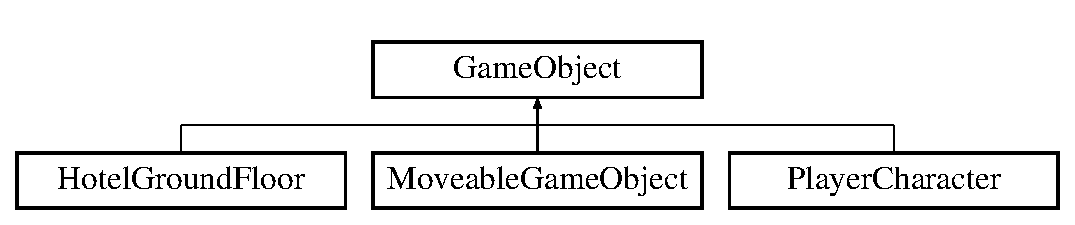
\includegraphics[height=2cm]{classGameObject}
\end{center}
\end{figure}
\subsection*{Public Member Functions}
\begin{DoxyCompactItemize}
\item 
\hyperlink{classGameObject_ad8d1bdb3864097a3723ddac03b947f95}{GameObject} (\hyperlink{classWorld}{World} $\ast$, CL\_\-Pointd \&, CL\_\-Angle \&)
\item 
void \hyperlink{classGameObject_a0eabb72240499a1878b420b5c3f0ecf3}{setDirection} (CL\_\-Angle \&)
\item 
CL\_\-Angle \hyperlink{classGameObject_a456901f9f0b261b206db248960633e50}{getDirection} (void)
\item 
void \hyperlink{classGameObject_a4fd1eeb91d5a220dde7b8574be19b651}{setPosition} (CL\_\-Pointd \&)
\item 
CL\_\-Pointd \hyperlink{classGameObject_adfc89f23ef6d0819c183f1c26bb27e58}{getPosition} (void)
\item 
virtual void \hyperlink{classGameObject_abb64143e72358beb808db22182517802}{draw} ()
\item 
virtual bool \hyperlink{classGameObject_ad2f3cd5d1f5a11b237507cd3ee98b95d}{update} (unsigned int)
\end{DoxyCompactItemize}
\subsection*{Protected Attributes}
\begin{DoxyCompactItemize}
\item 
\hypertarget{classGameObject_adce5bc0f31d7ce307f6bf8fe57030a24}{
\hyperlink{classWorld}{World} $\ast$ {\bfseries world}}
\label{classGameObject_adce5bc0f31d7ce307f6bf8fe57030a24}

\item 
\hypertarget{classGameObject_a9e3a44174a06dd260412d7a13d639d99}{
CL\_\-Pointd {\bfseries position}}
\label{classGameObject_a9e3a44174a06dd260412d7a13d639d99}

\item 
\hypertarget{classGameObject_a8df0dc007367b180dfcd9d2f193f6bdf}{
CL\_\-Angle {\bfseries direction}}
\label{classGameObject_a8df0dc007367b180dfcd9d2f193f6bdf}

\item 
\hypertarget{classGameObject_a5b841978ecf469bc3a69c0d05ad81013}{
CL\_\-Sprite $\ast$ {\bfseries static\_\-sprites} \mbox{[}8\mbox{]}}
\label{classGameObject_a5b841978ecf469bc3a69c0d05ad81013}

\item 
\hypertarget{classGameObject_a22464434abaabf3fb9aab0664dd22eb5}{
CL\_\-Sprite $\ast$ {\bfseries static\_\-current}}
\label{classGameObject_a22464434abaabf3fb9aab0664dd22eb5}

\end{DoxyCompactItemize}


\subsection{Constructor \& Destructor Documentation}
\hypertarget{classGameObject_ad8d1bdb3864097a3723ddac03b947f95}{
\index{GameObject@{GameObject}!GameObject@{GameObject}}
\index{GameObject@{GameObject}!GameObject@{GameObject}}
\subsubsection[{GameObject}]{\setlength{\rightskip}{0pt plus 5cm}GameObject::GameObject ({\bf World} $\ast$ {\em w}, \/  CL\_\-Pointd \& {\em initial\_\-position}, \/  CL\_\-Angle \& {\em initial\_\-direction})}}
\label{classGameObject_ad8d1bdb3864097a3723ddac03b947f95}
param w World$\ast$ param initial\_\-position CL\_\-Pointd The starting position in world coordinates. param initial\_\-direction CL\_\-Angle 

\subsection{Member Function Documentation}
\hypertarget{classGameObject_abb64143e72358beb808db22182517802}{
\index{GameObject@{GameObject}!draw@{draw}}
\index{draw@{draw}!GameObject@{GameObject}}
\subsubsection[{draw}]{\setlength{\rightskip}{0pt plus 5cm}void GameObject::draw (void)\hspace{0.3cm}{\ttfamily  \mbox{[}virtual\mbox{]}}}}
\label{classGameObject_abb64143e72358beb808db22182517802}
Draws the current static sprite for the object. 

Reimplemented in \hyperlink{classMoveableGameObject_a6110e3bcfb088cfaa53bc81ce220bab1}{MoveableGameObject}.\hypertarget{classGameObject_a456901f9f0b261b206db248960633e50}{
\index{GameObject@{GameObject}!getDirection@{getDirection}}
\index{getDirection@{getDirection}!GameObject@{GameObject}}
\subsubsection[{getDirection}]{\setlength{\rightskip}{0pt plus 5cm}CL\_\-Angle GameObject::getDirection (void)}}
\label{classGameObject_a456901f9f0b261b206db248960633e50}
Returns the angle. \hypertarget{classGameObject_adfc89f23ef6d0819c183f1c26bb27e58}{
\index{GameObject@{GameObject}!getPosition@{getPosition}}
\index{getPosition@{getPosition}!GameObject@{GameObject}}
\subsubsection[{getPosition}]{\setlength{\rightskip}{0pt plus 5cm}CL\_\-Pointd GameObject::getPosition (void)}}
\label{classGameObject_adfc89f23ef6d0819c183f1c26bb27e58}
Returns the position in world co-\/ordinates in CL\_\-Pointd. \hypertarget{classGameObject_a0eabb72240499a1878b420b5c3f0ecf3}{
\index{GameObject@{GameObject}!setDirection@{setDirection}}
\index{setDirection@{setDirection}!GameObject@{GameObject}}
\subsubsection[{setDirection}]{\setlength{\rightskip}{0pt plus 5cm}void GameObject::setDirection (CL\_\-Angle \& {\em new\_\-direction})}}
\label{classGameObject_a0eabb72240499a1878b420b5c3f0ecf3}
Sets the direction the game object is facing. This effects the sprite which is used when drawing it. \hypertarget{classGameObject_a4fd1eeb91d5a220dde7b8574be19b651}{
\index{GameObject@{GameObject}!setPosition@{setPosition}}
\index{setPosition@{setPosition}!GameObject@{GameObject}}
\subsubsection[{setPosition}]{\setlength{\rightskip}{0pt plus 5cm}void GameObject::setPosition (CL\_\-Pointd \& {\em new\_\-position})}}
\label{classGameObject_a4fd1eeb91d5a220dde7b8574be19b651}
Sets the position of the object.

param new\_\-position The position as CL\_\-Pointd in terms of world co-\/ordinates. \hypertarget{classGameObject_ad2f3cd5d1f5a11b237507cd3ee98b95d}{
\index{GameObject@{GameObject}!update@{update}}
\index{update@{update}!GameObject@{GameObject}}
\subsubsection[{update}]{\setlength{\rightskip}{0pt plus 5cm}bool GameObject::update (unsigned int {\em time\_\-elapsed\_\-ms})\hspace{0.3cm}{\ttfamily  \mbox{[}virtual\mbox{]}}}}
\label{classGameObject_ad2f3cd5d1f5a11b237507cd3ee98b95d}
Updates any animation in the current sprite. 

Reimplemented in \hyperlink{classMoveableGameObject_af2a5d981743e85b4bd35a90f874b361b}{MoveableGameObject}.

The documentation for this class was generated from the following files:\begin{DoxyCompactItemize}
\item 
source/game/\hyperlink{GameObject_8h}{GameObject.h}\item 
source/game/\hyperlink{GameObject_8cpp}{GameObject.cpp}\end{DoxyCompactItemize}

\hypertarget{classHotelGroundFloor}{
\section{HotelGroundFloor Class Reference}
\label{classHotelGroundFloor}\index{HotelGroundFloor@{HotelGroundFloor}}
}
Inheritance diagram for HotelGroundFloor:\begin{figure}[H]
\begin{center}
\leavevmode
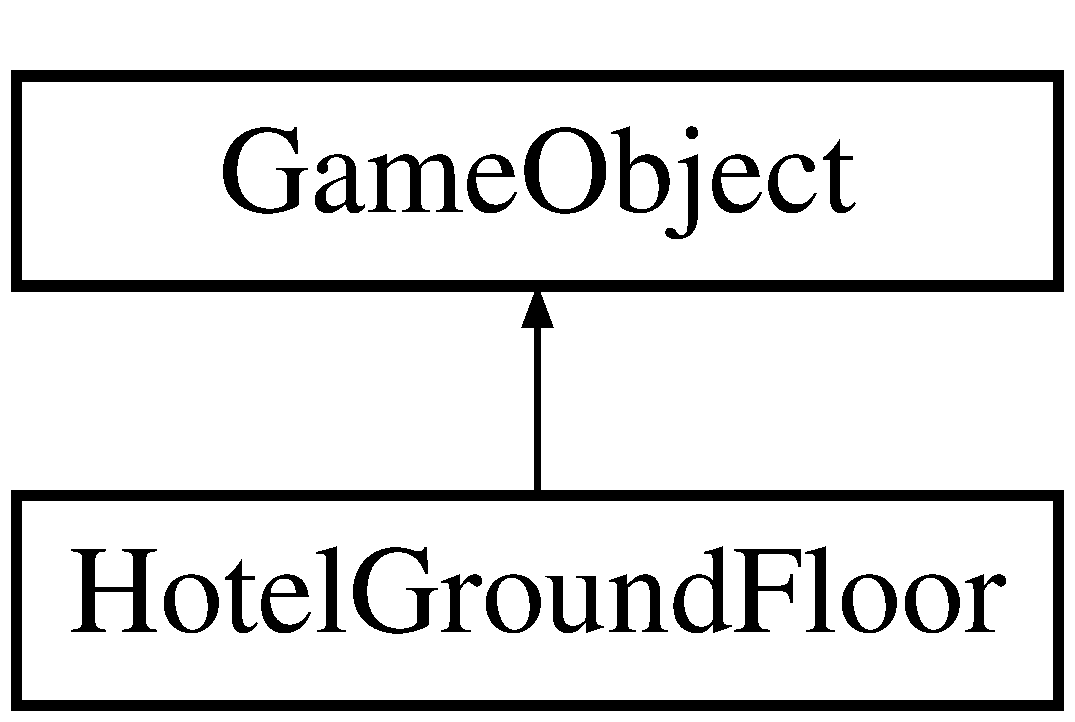
\includegraphics[height=2cm]{classHotelGroundFloor}
\end{center}
\end{figure}
\subsection*{Public Member Functions}
\begin{DoxyCompactItemize}
\item 
\hypertarget{classHotelGroundFloor_a3feeaf0aee35b8cd060bf8c21375dff9}{
{\bfseries HotelGroundFloor} (\hyperlink{classScene}{Scene} $\ast$, CL\_\-Pointd \&, CL\_\-Angle \&)}
\label{classHotelGroundFloor_a3feeaf0aee35b8cd060bf8c21375dff9}

\item 
bool \hyperlink{classHotelGroundFloor_a654f889fe9e9d275f2bfee99bef50b76}{update} (unsigned int)
\end{DoxyCompactItemize}


\subsection{Member Function Documentation}
\hypertarget{classHotelGroundFloor_a654f889fe9e9d275f2bfee99bef50b76}{
\index{HotelGroundFloor@{HotelGroundFloor}!update@{update}}
\index{update@{update}!HotelGroundFloor@{HotelGroundFloor}}
\subsubsection[{update}]{\setlength{\rightskip}{0pt plus 5cm}bool HotelGroundFloor::update (unsigned int {\em time\_\-elapsed\_\-ms})\hspace{0.3cm}{\ttfamily  \mbox{[}virtual\mbox{]}}}}
\label{classHotelGroundFloor_a654f889fe9e9d275f2bfee99bef50b76}
Updates any animation in the current sprite. 

Reimplemented from \hyperlink{classGameObject_ad2f3cd5d1f5a11b237507cd3ee98b95d}{GameObject}.



The documentation for this class was generated from the following files:\begin{DoxyCompactItemize}
\item 
source/game/game\_\-objects/HotelGroundFloor.h\item 
source/game/game\_\-objects/HotelGroundFloor.cpp\end{DoxyCompactItemize}

\hypertarget{classIsometricGrid}{
\section{IsometricGrid Class Reference}
\label{classIsometricGrid}\index{IsometricGrid@{IsometricGrid}}
}


{\ttfamily \#include $<$IsometricGrid.h$>$}Inheritance diagram for IsometricGrid::\begin{figure}[H]
\begin{center}
\leavevmode
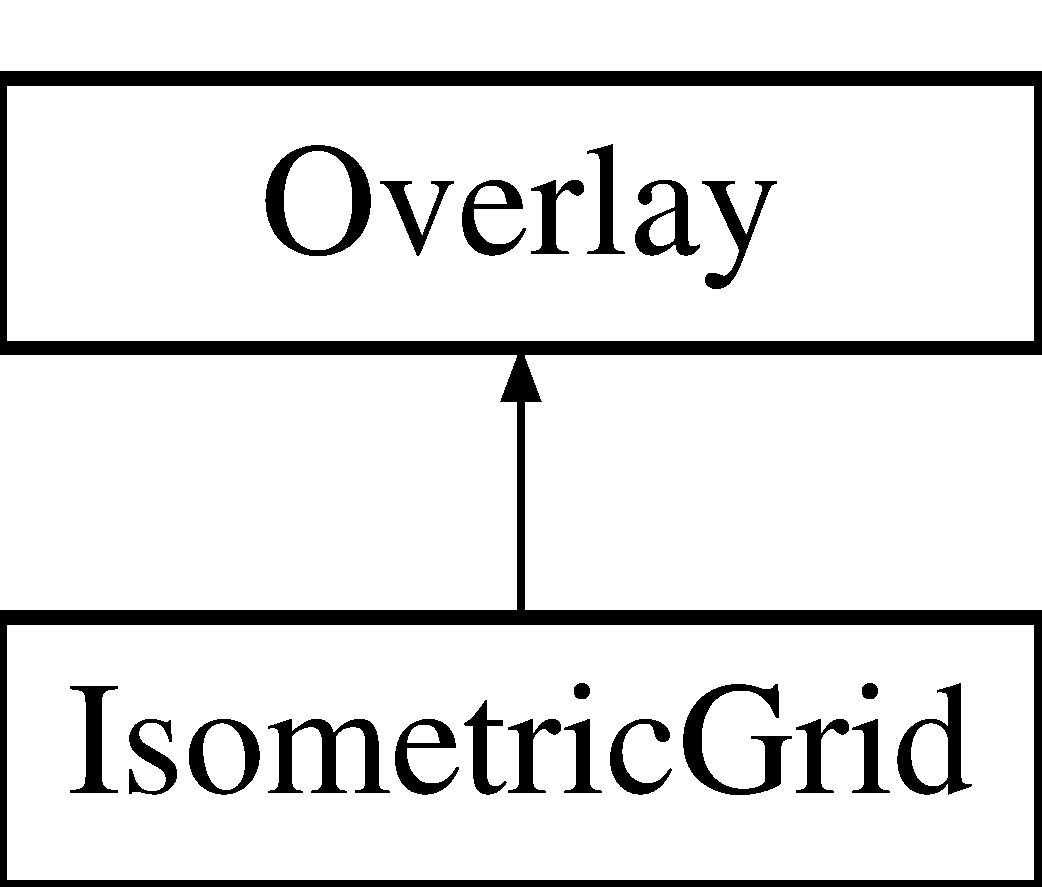
\includegraphics[height=2cm]{classIsometricGrid}
\end{center}
\end{figure}
\subsection*{Public Member Functions}
\begin{DoxyCompactItemize}
\item 
\hypertarget{classIsometricGrid_a4ac39773481a3937b415a71e8e7a29bd}{
{\bfseries IsometricGrid} (\hyperlink{classWorld}{World} $\ast$)}
\label{classIsometricGrid_a4ac39773481a3937b415a71e8e7a29bd}

\item 
\hypertarget{classIsometricGrid_a3138024ea901361f87a47c008fe4f31d}{
void {\bfseries draw} (void)}
\label{classIsometricGrid_a3138024ea901361f87a47c008fe4f31d}

\end{DoxyCompactItemize}


\subsection{Detailed Description}
Constructs a very basic 60x60 isometric grid overlay when calling the draw() function. 

The documentation for this class was generated from the following files:\begin{DoxyCompactItemize}
\item 
IsometricGrid.h\item 
IsometricGrid.cpp\end{DoxyCompactItemize}

\hypertarget{classMainMenu}{
\section{MainMenu Class Reference}
\label{classMainMenu}\index{MainMenu@{MainMenu}}
}
Inheritance diagram for MainMenu::\begin{figure}[H]
\begin{center}
\leavevmode
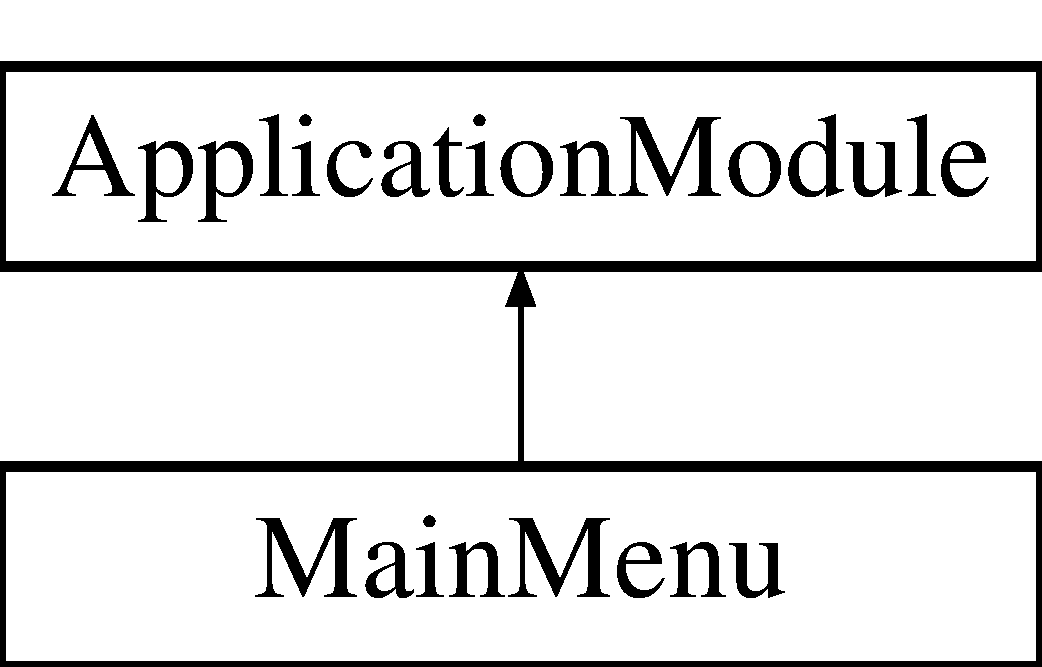
\includegraphics[height=2cm]{classMainMenu}
\end{center}
\end{figure}
\subsection*{Public Member Functions}
\begin{DoxyCompactItemize}
\item 
\hypertarget{classMainMenu_a4f8cb7bce56b9c1053ad0257fa8bec3a}{
{\bfseries MainMenu} (CL\_\-DisplayWindow \&)}
\label{classMainMenu_a4f8cb7bce56b9c1053ad0257fa8bec3a}

\end{DoxyCompactItemize}


The documentation for this class was generated from the following files:\begin{DoxyCompactItemize}
\item 
source/main\_\-menu/\hyperlink{MainMenu_8h}{MainMenu.h}\item 
source/main\_\-menu/\hyperlink{MainMenu_8cpp}{MainMenu.cpp}\end{DoxyCompactItemize}

\hypertarget{classMonster}{
\section{Monster Class Reference}
\label{classMonster}\index{Monster@{Monster}}
}
\subsection*{Public Member Functions}
\begin{DoxyCompactItemize}
\item 
\hyperlink{classMonster_af4dbf8422477e5d7a8c8639ed8a6e7a7}{Monster} (CL\_\-Pointf, \hyperlink{classMonsterGeneratorDemo}{MonsterGeneratorDemo} $\ast$)
\item 
\hypertarget{classMonster_a6de8e0eb90db5e6005dd7e26dc37cf04}{
{\bfseries Monster} (CL\_\-Pointf, \hyperlink{classMonsterGeneratorDemo}{MonsterGeneratorDemo} $\ast$, std::map$<$ CL\_\-String8, CL\_\-String8 $>$)}
\label{classMonster_a6de8e0eb90db5e6005dd7e26dc37cf04}

\item 
\hyperlink{classMonster_a1b3329ad00743bd5432d81ee487ca7ae}{Monster} (CL\_\-Pointf, \hyperlink{classMonsterGeneratorDemo}{MonsterGeneratorDemo} $\ast$, \hyperlink{classBBN__Plot}{BBN\_\-Plot} $\ast$)
\item 
\hypertarget{classMonster_aaf16974cdf557c0e62e445c94ddcfc53}{
void {\bfseries draw} (CL\_\-GraphicContext $\ast$gc)}
\label{classMonster_aaf16974cdf557c0e62e445c94ddcfc53}

\end{DoxyCompactItemize}
\subsection*{Protected Member Functions}
\begin{DoxyCompactItemize}
\item 
\hypertarget{classMonster_a3e1c502f98e13fef189adb45631f4ca2}{
void {\bfseries load\_\-sprites} (void)}
\label{classMonster_a3e1c502f98e13fef189adb45631f4ca2}

\end{DoxyCompactItemize}
\subsection*{Protected Attributes}
\begin{DoxyCompactItemize}
\item 
\hypertarget{classMonster_a74d6adb21c6a59f1444f52f8645d186b}{
CL\_\-Sprite {\bfseries \_\-legs}}
\label{classMonster_a74d6adb21c6a59f1444f52f8645d186b}

\item 
\hypertarget{classMonster_aedc760e23fe73e5f6e4936cf23639b8c}{
CL\_\-Sprite {\bfseries \_\-body}}
\label{classMonster_aedc760e23fe73e5f6e4936cf23639b8c}

\item 
\hypertarget{classMonster_aad50e8f3e9c8ec0f4b236796e474092f}{
CL\_\-Sprite {\bfseries \_\-mouth}}
\label{classMonster_aad50e8f3e9c8ec0f4b236796e474092f}

\item 
\hypertarget{classMonster_aa21f28b1d669df2750b0ac8cac4b1d3a}{
CL\_\-Sprite {\bfseries \_\-eyes}}
\label{classMonster_aa21f28b1d669df2750b0ac8cac4b1d3a}

\item 
\hypertarget{classMonster_ae74ed89492b52a6bc2b7eceb91f68b33}{
CL\_\-Sprite {\bfseries \_\-arms}}
\label{classMonster_ae74ed89492b52a6bc2b7eceb91f68b33}

\item 
\hypertarget{classMonster_af7d855b6b8b4967751381ebc36a78619}{
CL\_\-Sprite {\bfseries \_\-background}}
\label{classMonster_af7d855b6b8b4967751381ebc36a78619}

\item 
\hypertarget{classMonster_af888771b6f7e506b206cdf7c0684d6e3}{
CL\_\-Sprite {\bfseries \_\-extra}}
\label{classMonster_af888771b6f7e506b206cdf7c0684d6e3}

\item 
\hypertarget{classMonster_a9081e7e2f5dcc47012c4a03d14c1d921}{
CL\_\-Rectf {\bfseries \_\-destination}}
\label{classMonster_a9081e7e2f5dcc47012c4a03d14c1d921}

\item 
\hypertarget{classMonster_a31e59d9fe5c537980856149cce2d47da}{
\hyperlink{classBBN__Plot}{BBN\_\-Plot} $\ast$ {\bfseries \_\-properties}}
\label{classMonster_a31e59d9fe5c537980856149cce2d47da}

\item 
\hypertarget{classMonster_a3213f8da9db9f30ac68a73fa89e82569}{
\hyperlink{classMonsterGeneratorDemo}{MonsterGeneratorDemo} $\ast$ {\bfseries \_\-parent}}
\label{classMonster_a3213f8da9db9f30ac68a73fa89e82569}

\end{DoxyCompactItemize}


\subsection{Constructor \& Destructor Documentation}
\hypertarget{classMonster_af4dbf8422477e5d7a8c8639ed8a6e7a7}{
\index{Monster@{Monster}!Monster@{Monster}}
\index{Monster@{Monster}!Monster@{Monster}}
\subsubsection[{Monster}]{\setlength{\rightskip}{0pt plus 5cm}Monster::Monster (CL\_\-Pointf {\em location}, \/  {\bf MonsterGeneratorDemo} $\ast$ {\em parent})}}
\label{classMonster_af4dbf8422477e5d7a8c8639ed8a6e7a7}
Loads the Bayes net for the object and sets the sprites to use for each of the body components. \hypertarget{classMonster_a1b3329ad00743bd5432d81ee487ca7ae}{
\index{Monster@{Monster}!Monster@{Monster}}
\index{Monster@{Monster}!Monster@{Monster}}
\subsubsection[{Monster}]{\setlength{\rightskip}{0pt plus 5cm}Monster::Monster (CL\_\-Pointf {\em location}, \/  {\bf MonsterGeneratorDemo} $\ast$ {\em parent}, \/  {\bf BBN\_\-Plot} $\ast$ {\em bbn})}}
\label{classMonster_a1b3329ad00743bd5432d81ee487ca7ae}
Generates monster from the provided bayes net. Makes a copy. 

The documentation for this class was generated from the following files:\begin{DoxyCompactItemize}
\item 
source/monster\_\-generator\_\-demo/Monster.h\item 
source/monster\_\-generator\_\-demo/Monster.cpp\end{DoxyCompactItemize}

\hypertarget{classMonsterGeneratorDemo}{
\section{MonsterGeneratorDemo Class Reference}
\label{classMonsterGeneratorDemo}\index{MonsterGeneratorDemo@{MonsterGeneratorDemo}}
}


{\ttfamily \#include $<$MonsterGeneratorDemo.h$>$}

Inheritance diagram for MonsterGeneratorDemo:\begin{figure}[H]
\begin{center}
\leavevmode
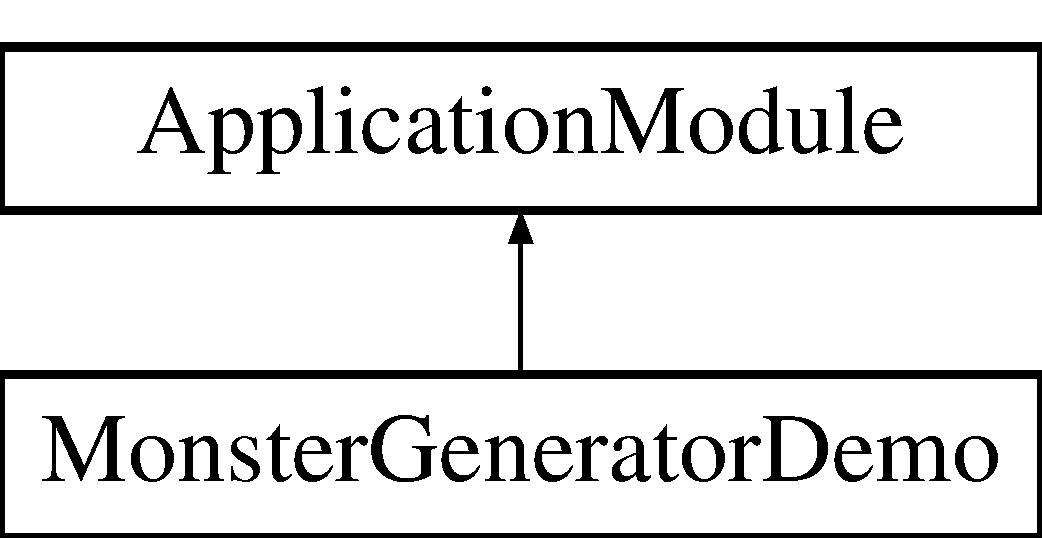
\includegraphics[height=2cm]{classMonsterGeneratorDemo}
\end{center}
\end{figure}
\subsection*{Public Member Functions}
\begin{DoxyCompactItemize}
\item 
\hypertarget{classMonsterGeneratorDemo_a9b2e81516e469825a83fa54586641dbb}{
{\bfseries MonsterGeneratorDemo} (const CL\_\-DisplayWindow \&)}
\label{classMonsterGeneratorDemo_a9b2e81516e469825a83fa54586641dbb}

\item 
\hypertarget{classMonsterGeneratorDemo_a375c1a42ba5cbae38ce983e238d0ce03}{
CL\_\-ResourceManager $\ast$ {\bfseries get\_\-rm} (void)}
\label{classMonsterGeneratorDemo_a375c1a42ba5cbae38ce983e238d0ce03}

\end{DoxyCompactItemize}
\subsection*{Protected Member Functions}
\begin{DoxyCompactItemize}
\item 
\hypertarget{classMonsterGeneratorDemo_a6f66d4ed6f4d0a4ba96f96edac2fedb1}{
void {\bfseries draw} (void)}
\label{classMonsterGeneratorDemo_a6f66d4ed6f4d0a4ba96f96edac2fedb1}

\item 
void \hyperlink{classMonsterGeneratorDemo_a9f7a998bfd08409c3db44c755d50721f}{generate\_\-monster} (void)
\item 
\hypertarget{classMonsterGeneratorDemo_ae1ad1c6c81b5e1c18ebccaa5b661e360}{
void {\bfseries update} (void)}
\label{classMonsterGeneratorDemo_ae1ad1c6c81b5e1c18ebccaa5b661e360}

\item 
void \hyperlink{classMonsterGeneratorDemo_a79a6136789c43d0a1502b7ad0381079a}{show\_\-editor} (void)
\item 
bool \hyperlink{classMonsterGeneratorDemo_a81a9869082eb20376f4a53723d805bfa}{close\_\-editor} (void)
\item 
\hypertarget{classMonsterGeneratorDemo_a2cf5ccbf2f89c759875428998fa1bf5b}{
virtual void {\bfseries on\_\-key\_\-down} (const CL\_\-InputEvent \&key, const CL\_\-InputState \&state)}
\label{classMonsterGeneratorDemo_a2cf5ccbf2f89c759875428998fa1bf5b}

\item 
CL\_\-Pointf \hyperlink{classMonsterGeneratorDemo_a82938578e271b99cb300c6a668dff550}{get\_\-next\_\-monster\_\-position} (void)
\end{DoxyCompactItemize}
\subsection*{Protected Attributes}
\begin{DoxyCompactItemize}
\item 
\hypertarget{classMonsterGeneratorDemo_aed1250d417ea668cae0719d8b1f5dd13}{
CL\_\-ResourceManager {\bfseries \_\-rm}}
\label{classMonsterGeneratorDemo_aed1250d417ea668cae0719d8b1f5dd13}

\item 
\hypertarget{classMonsterGeneratorDemo_ab06ee3e4a2b74beb7de00bc7af7a2cd2}{
std::list$<$ \hyperlink{classMonster}{Monster} $\ast$ $>$ {\bfseries \_\-monsters}}
\label{classMonsterGeneratorDemo_ab06ee3e4a2b74beb7de00bc7af7a2cd2}

\item 
\hypertarget{classMonsterGeneratorDemo_ac1f9b1e72a1e36d98f1dfe3af44c675f}{
CL\_\-Window $\ast$ {\bfseries \_\-window\_\-editor}}
\label{classMonsterGeneratorDemo_ac1f9b1e72a1e36d98f1dfe3af44c675f}

\item 
\hypertarget{classMonsterGeneratorDemo_a250a4cddf3123722f19de1dc7478b838}{
\hyperlink{classBBN__Info}{BBN\_\-Info} $\ast$ {\bfseries \_\-control\_\-bbn}}
\label{classMonsterGeneratorDemo_a250a4cddf3123722f19de1dc7478b838}

\item 
\hypertarget{classMonsterGeneratorDemo_a7ce77640c29d0a414061db6f0ab47310}{
\hyperlink{classBBN__Plot}{BBN\_\-Plot} $\ast$ {\bfseries \_\-active\_\-net}}
\label{classMonsterGeneratorDemo_a7ce77640c29d0a414061db6f0ab47310}

\item 
\hypertarget{classMonsterGeneratorDemo_aa9658c30603874a9eb5de77e40f83ac6}{
CL\_\-PushButton $\ast$ {\bfseries \_\-button\_\-generate}}
\label{classMonsterGeneratorDemo_aa9658c30603874a9eb5de77e40f83ac6}

\item 
\hypertarget{classMonsterGeneratorDemo_a6c01d36ed849f6e74429cb086a7c783b}{
int {\bfseries \_\-next\_\-monster\_\-x}}
\label{classMonsterGeneratorDemo_a6c01d36ed849f6e74429cb086a7c783b}

\item 
\hypertarget{classMonsterGeneratorDemo_acc504c13da359f9c4a8efc80288efab5}{
int {\bfseries \_\-next\_\-monster\_\-y}}
\label{classMonsterGeneratorDemo_acc504c13da359f9c4a8efc80288efab5}

\end{DoxyCompactItemize}


\subsection{Detailed Description}
The monster generator demo aims to test how Bayes nets can be use to determine cohesive properties of randomly generated objects. In this case monsters. Each time the object is instantiated so is a Bayes network and from this a new kind of monster is generated. 

\subsection{Member Function Documentation}
\hypertarget{classMonsterGeneratorDemo_a81a9869082eb20376f4a53723d805bfa}{
\index{MonsterGeneratorDemo@{MonsterGeneratorDemo}!close\_\-editor@{close\_\-editor}}
\index{close\_\-editor@{close\_\-editor}!MonsterGeneratorDemo@{MonsterGeneratorDemo}}
\subsubsection[{close\_\-editor}]{\setlength{\rightskip}{0pt plus 5cm}bool MonsterGeneratorDemo::close\_\-editor (void)\hspace{0.3cm}{\ttfamily  \mbox{[}protected\mbox{]}}}}
\label{classMonsterGeneratorDemo_a81a9869082eb20376f4a53723d805bfa}
Closes the active editor window and components.

\begin{DoxyReturn}{Returns}

\end{DoxyReturn}
\hypertarget{classMonsterGeneratorDemo_a9f7a998bfd08409c3db44c755d50721f}{
\index{MonsterGeneratorDemo@{MonsterGeneratorDemo}!generate\_\-monster@{generate\_\-monster}}
\index{generate\_\-monster@{generate\_\-monster}!MonsterGeneratorDemo@{MonsterGeneratorDemo}}
\subsubsection[{generate\_\-monster}]{\setlength{\rightskip}{0pt plus 5cm}void MonsterGeneratorDemo::generate\_\-monster (void)\hspace{0.3cm}{\ttfamily  \mbox{[}protected\mbox{]}}}}
\label{classMonsterGeneratorDemo_a9f7a998bfd08409c3db44c755d50721f}
Uses the bayes net represented in \_\-control\_\-bbn to generate a monster and display it on the screen. \hypertarget{classMonsterGeneratorDemo_a82938578e271b99cb300c6a668dff550}{
\index{MonsterGeneratorDemo@{MonsterGeneratorDemo}!get\_\-next\_\-monster\_\-position@{get\_\-next\_\-monster\_\-position}}
\index{get\_\-next\_\-monster\_\-position@{get\_\-next\_\-monster\_\-position}!MonsterGeneratorDemo@{MonsterGeneratorDemo}}
\subsubsection[{get\_\-next\_\-monster\_\-position}]{\setlength{\rightskip}{0pt plus 5cm}CL\_\-Pointf MonsterGeneratorDemo::get\_\-next\_\-monster\_\-position (void)\hspace{0.3cm}{\ttfamily  \mbox{[}protected\mbox{]}}}}
\label{classMonsterGeneratorDemo_a82938578e271b99cb300c6a668dff550}
Returns the next grid location spare to place a generated monster.

\begin{DoxyReturn}{Returns}

\end{DoxyReturn}
\hypertarget{classMonsterGeneratorDemo_a79a6136789c43d0a1502b7ad0381079a}{
\index{MonsterGeneratorDemo@{MonsterGeneratorDemo}!show\_\-editor@{show\_\-editor}}
\index{show\_\-editor@{show\_\-editor}!MonsterGeneratorDemo@{MonsterGeneratorDemo}}
\subsubsection[{show\_\-editor}]{\setlength{\rightskip}{0pt plus 5cm}void MonsterGeneratorDemo::show\_\-editor (void)\hspace{0.3cm}{\ttfamily  \mbox{[}protected\mbox{]}}}}
\label{classMonsterGeneratorDemo_a79a6136789c43d0a1502b7ad0381079a}
Creates the monster bayes net editor window if one doesn't already exit and ensures it is visible if one does. 

The documentation for this class was generated from the following files:\begin{DoxyCompactItemize}
\item 
source/monster\_\-generator\_\-demo/MonsterGeneratorDemo.h\item 
source/monster\_\-generator\_\-demo/MonsterGeneratorDemo.cpp\end{DoxyCompactItemize}

\hypertarget{classMoveableGameObject}{
\section{MoveableGameObject Class Reference}
\label{classMoveableGameObject}\index{MoveableGameObject@{MoveableGameObject}}
}
Inheritance diagram for MoveableGameObject::\begin{figure}[H]
\begin{center}
\leavevmode
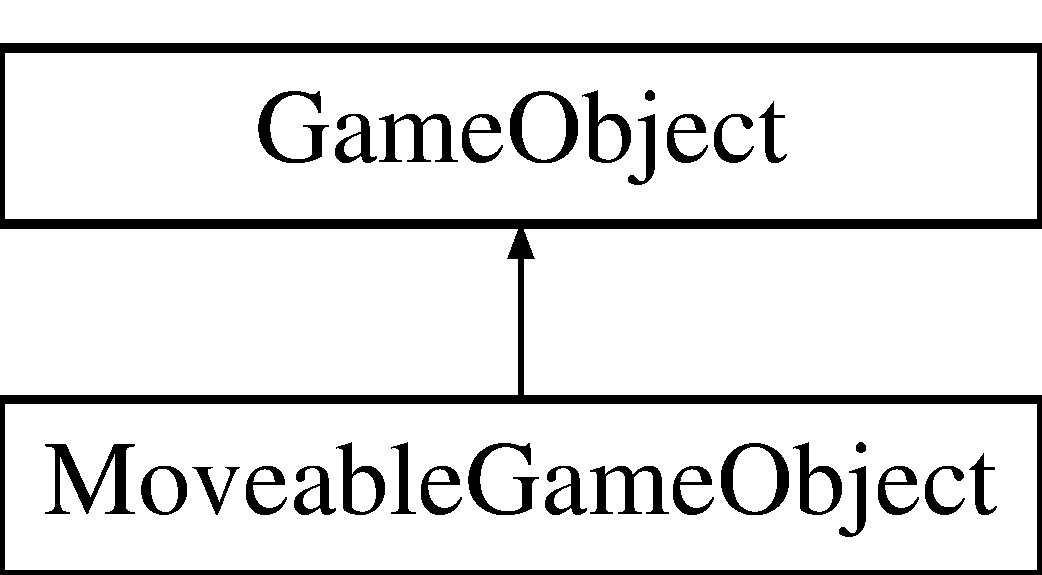
\includegraphics[height=2cm]{classMoveableGameObject}
\end{center}
\end{figure}
\subsection*{Public Member Functions}
\begin{DoxyCompactItemize}
\item 
void \hyperlink{classMoveableGameObject_a6110e3bcfb088cfaa53bc81ce220bab1}{draw} (void)
\item 
bool \hyperlink{classMoveableGameObject_af2a5d981743e85b4bd35a90f874b361b}{update} (unsigned int)
\item 
\hypertarget{classMoveableGameObject_a35e6de5de69921201d48989af9310b71}{
{\bfseries MoveableGameObject} (\hyperlink{classWorld}{World} $\ast$, CL\_\-Pointd \&, CL\_\-Angle \&)}
\label{classMoveableGameObject_a35e6de5de69921201d48989af9310b71}

\end{DoxyCompactItemize}


\subsection{Member Function Documentation}
\hypertarget{classMoveableGameObject_a6110e3bcfb088cfaa53bc81ce220bab1}{
\index{MoveableGameObject@{MoveableGameObject}!draw@{draw}}
\index{draw@{draw}!MoveableGameObject@{MoveableGameObject}}
\subsubsection[{draw}]{\setlength{\rightskip}{0pt plus 5cm}void MoveableGameObject::draw (void)\hspace{0.3cm}{\ttfamily  \mbox{[}virtual\mbox{]}}}}
\label{classMoveableGameObject_a6110e3bcfb088cfaa53bc81ce220bab1}
Draws the current static sprite for the object. 

Reimplemented from \hyperlink{classGameObject_abb64143e72358beb808db22182517802}{GameObject}.\hypertarget{classMoveableGameObject_af2a5d981743e85b4bd35a90f874b361b}{
\index{MoveableGameObject@{MoveableGameObject}!update@{update}}
\index{update@{update}!MoveableGameObject@{MoveableGameObject}}
\subsubsection[{update}]{\setlength{\rightskip}{0pt plus 5cm}bool MoveableGameObject::update (unsigned int {\em time\_\-elapsed\_\-ms})\hspace{0.3cm}{\ttfamily  \mbox{[}virtual\mbox{]}}}}
\label{classMoveableGameObject_af2a5d981743e85b4bd35a90f874b361b}
Updates any animation in the current sprite. 

Reimplemented from \hyperlink{classGameObject_ad2f3cd5d1f5a11b237507cd3ee98b95d}{GameObject}.

The documentation for this class was generated from the following files:\begin{DoxyCompactItemize}
\item 
source/game/\hyperlink{MoveableGameObject_8h}{MoveableGameObject.h}\item 
source/game/\hyperlink{MoveableGameObject_8cpp}{MoveableGameObject.cpp}\end{DoxyCompactItemize}

\hypertarget{classOverlay}{
\section{Overlay Class Reference}
\label{classOverlay}\index{Overlay@{Overlay}}
}
Inheritance diagram for Overlay:\begin{figure}[H]
\begin{center}
\leavevmode
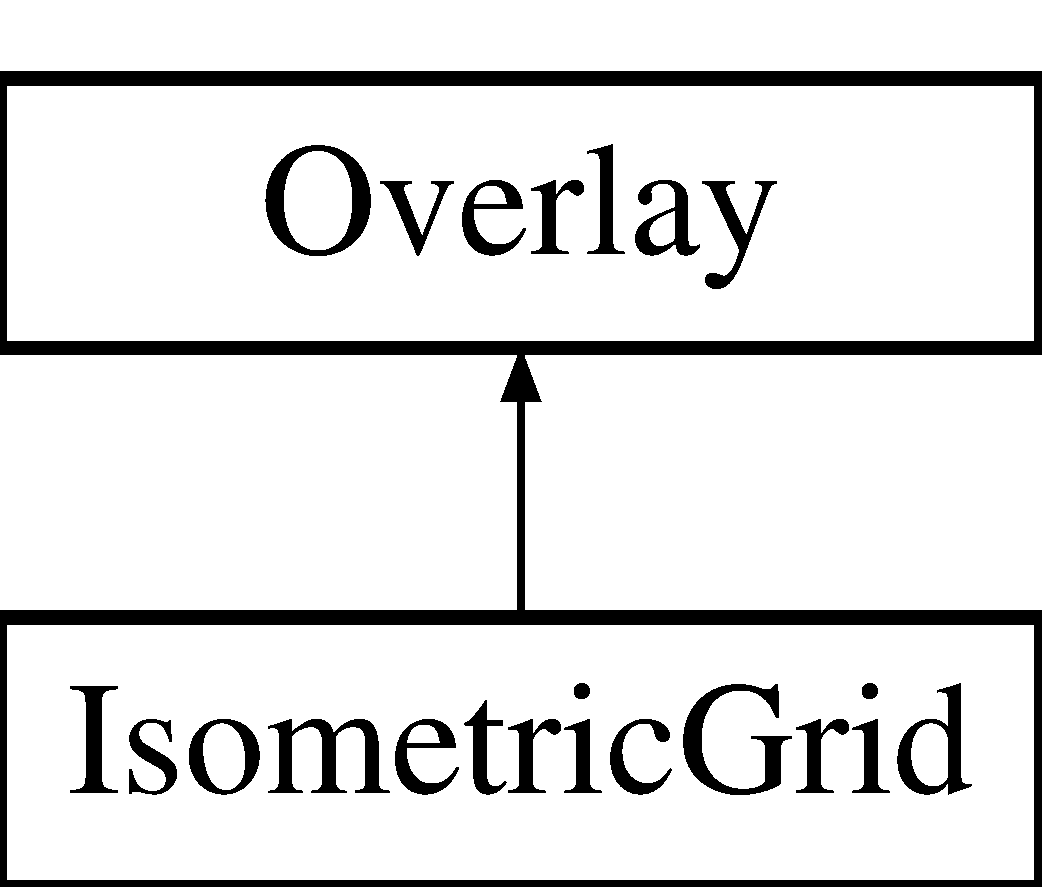
\includegraphics[height=2cm]{classOverlay}
\end{center}
\end{figure}
\subsection*{Public Member Functions}
\begin{DoxyCompactItemize}
\item 
\hypertarget{classOverlay_aecb2ad2cea6041a1b1e332e041daeb13}{
{\bfseries Overlay} (\hyperlink{classWorld}{World} $\ast$)}
\label{classOverlay_aecb2ad2cea6041a1b1e332e041daeb13}

\item 
\hypertarget{classOverlay_a384639128697df8c44c3801ae9212be3}{
virtual void {\bfseries draw} ()=0}
\label{classOverlay_a384639128697df8c44c3801ae9212be3}

\end{DoxyCompactItemize}
\subsection*{Protected Attributes}
\begin{DoxyCompactItemize}
\item 
\hypertarget{classOverlay_aa0de2439856791f770c9e2e9bdc5b613}{
\hyperlink{classWorld}{World} $\ast$ {\bfseries world}}
\label{classOverlay_aa0de2439856791f770c9e2e9bdc5b613}

\end{DoxyCompactItemize}


The documentation for this class was generated from the following files:\begin{DoxyCompactItemize}
\item 
source/game/\hyperlink{Overlay_8h}{Overlay.h}\item 
source/game/\hyperlink{Overlay_8cpp}{Overlay.cpp}\end{DoxyCompactItemize}

\hypertarget{classPlayerCharacter}{
\section{PlayerCharacter Class Reference}
\label{classPlayerCharacter}\index{PlayerCharacter@{PlayerCharacter}}
}
Inheritance diagram for PlayerCharacter::\begin{figure}[H]
\begin{center}
\leavevmode
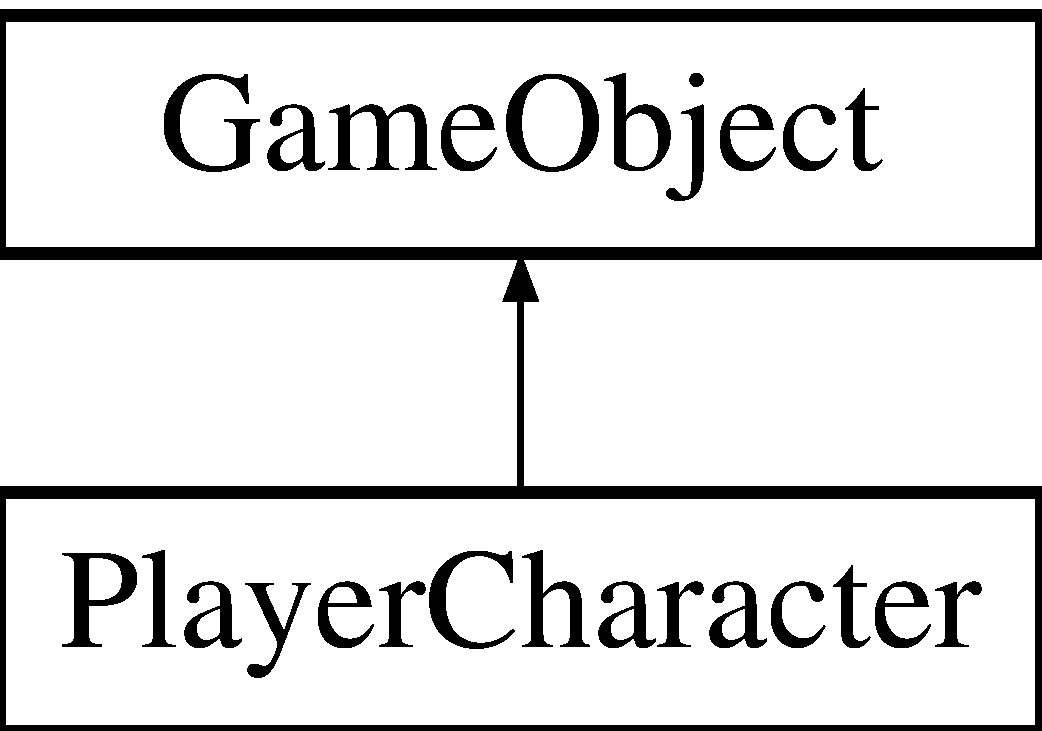
\includegraphics[height=2cm]{classPlayerCharacter}
\end{center}
\end{figure}
\subsection*{Public Member Functions}
\begin{DoxyCompactItemize}
\item 
\hypertarget{classPlayerCharacter_a0207723ef3dc387dcf80b01839715d31}{
{\bfseries PlayerCharacter} (\hyperlink{classWorld}{World} $\ast$, CL\_\-Pointd \&, CL\_\-Angle \&)}
\label{classPlayerCharacter_a0207723ef3dc387dcf80b01839715d31}

\end{DoxyCompactItemize}


The documentation for this class was generated from the following files:\begin{DoxyCompactItemize}
\item 
source/game/\hyperlink{PlayerCharacter_8h}{PlayerCharacter.h}\item 
source/game/\hyperlink{PlayerCharacter_8cpp}{PlayerCharacter.cpp}\end{DoxyCompactItemize}

\hypertarget{classProgram}{
\section{Program Class Reference}
\label{classProgram}\index{Program@{Program}}
}
\subsection*{Static Public Member Functions}
\begin{DoxyCompactItemize}
\item 
\hypertarget{classProgram_a97eed8197e64916a57f1d89477932d7a}{
static int {\bfseries main} (const std::vector$<$ CL\_\-String $>$ \&args)}
\label{classProgram_a97eed8197e64916a57f1d89477932d7a}

\end{DoxyCompactItemize}


The documentation for this class was generated from the following file:\begin{DoxyCompactItemize}
\item 
isometric.cpp\end{DoxyCompactItemize}

\hypertarget{classProp}{
\section{Prop Class Reference}
\label{classProp}\index{Prop@{Prop}}
}


The documentation for this class was generated from the following files:\begin{DoxyCompactItemize}
\item 
source/game/game\_\-objects/\hyperlink{Prop_8h}{Prop.h}\item 
source/game/game\_\-objects/\hyperlink{Prop_8cpp}{Prop.cpp}\end{DoxyCompactItemize}

\hypertarget{classRoom}{
\section{Room Class Reference}
\label{classRoom}\index{Room@{Room}}
}
Inheritance diagram for Room:\begin{figure}[H]
\begin{center}
\leavevmode
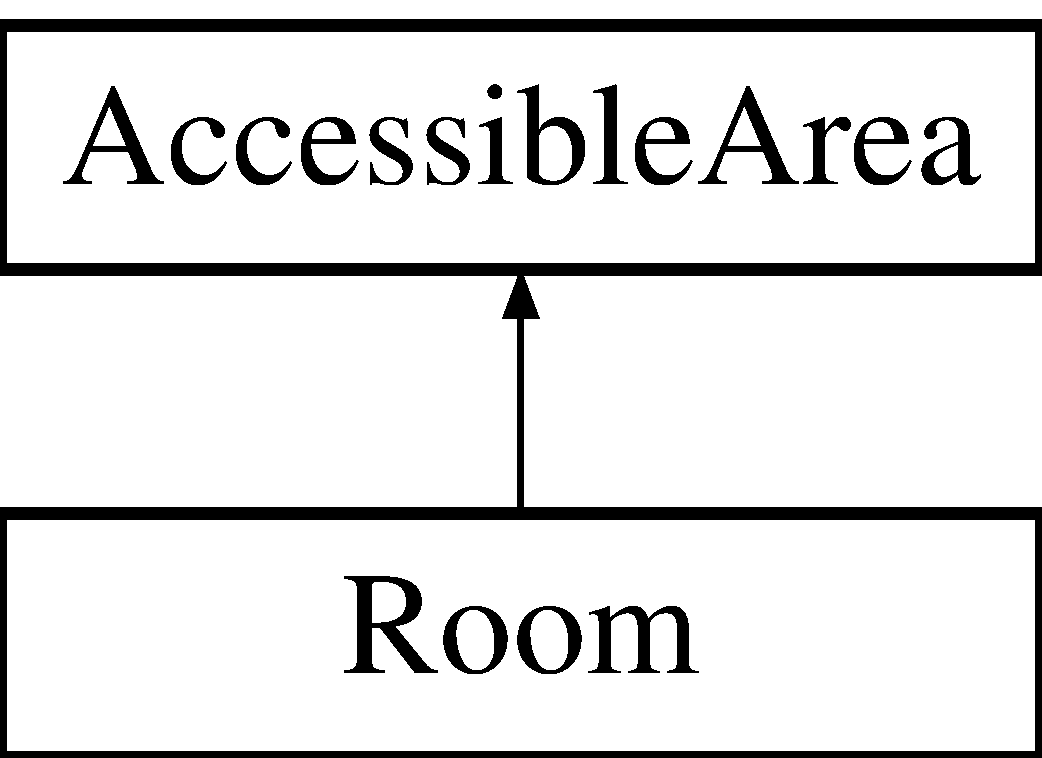
\includegraphics[height=2cm]{classRoom}
\end{center}
\end{figure}
\subsection*{Public Member Functions}
\begin{DoxyCompactItemize}
\item 
\hypertarget{classRoom_a063d845a90d110a4ef1672cd47d3bd70}{
{\bfseries Room} (\hyperlink{classScene}{Scene} $\ast$, const CL\_\-String8 \&, double, double, double, double)}
\label{classRoom_a063d845a90d110a4ef1672cd47d3bd70}

\item 
\hypertarget{classRoom_ac0b17aaf2c3e3c2e0aff771a7a2b7741}{
virtual void {\bfseries draw} (void)}
\label{classRoom_ac0b17aaf2c3e3c2e0aff771a7a2b7741}

\item 
\hypertarget{classRoom_aef0381c8b9ce884f3dcca64882ac06bb}{
CL\_\-String8 {\bfseries getName} (void)}
\label{classRoom_aef0381c8b9ce884f3dcca64882ac06bb}

\end{DoxyCompactItemize}
\subsection*{Protected Attributes}
\begin{DoxyCompactItemize}
\item 
\hypertarget{classRoom_ac583346cccae43f9fef8d484e2e084e6}{
CL\_\-String8 {\bfseries \_\-name}}
\label{classRoom_ac583346cccae43f9fef8d484e2e084e6}

\end{DoxyCompactItemize}


The documentation for this class was generated from the following files:\begin{DoxyCompactItemize}
\item 
source/game/\hyperlink{Room_8h}{Room.h}\item 
source/game/\hyperlink{Room_8cpp}{Room.cpp}\end{DoxyCompactItemize}

\hypertarget{classScene}{
\section{Scene Class Reference}
\label{classScene}\index{Scene@{Scene}}
}
\subsection*{Public Member Functions}
\begin{DoxyCompactItemize}
\item 
\hypertarget{classScene_a4eb3fdb166e0021e4e52fe19f9562183}{
{\bfseries Scene} (\hyperlink{classWorld}{World} $\ast$)}
\label{classScene_a4eb3fdb166e0021e4e52fe19f9562183}

\item 
\hypertarget{classScene_ac880d620e9331ee220eab871769bc26c}{
\hyperlink{classViewport}{Viewport} $\ast$ {\bfseries get\_\-active\_\-viewport} (void)}
\label{classScene_ac880d620e9331ee220eab871769bc26c}

\item 
\hypertarget{classScene_aca4855a051e9198608d26b6d9ae30cdb}{
\hyperlink{classWorld}{World} $\ast$ {\bfseries get\_\-world} (void)}
\label{classScene_aca4855a051e9198608d26b6d9ae30cdb}

\item 
void \hyperlink{classScene_af4940a9c9e62cb5ced3e7f5206d903a3}{add\_\-game\_\-object} (\hyperlink{classGameObject}{GameObject} $\ast$)
\item 
void \hyperlink{classScene_a41fbbe388ea322df338648e66611ffcf}{draw} (void)
\item 
void \hyperlink{classScene_a065d1b88078a09f2b77e80f663a40b2d}{update} (unsigned int)
\item 
\hypertarget{classScene_a8e146347a0f1dbe2231788a8d07d2746}{
void {\bfseries add\_\-viewport} (\hyperlink{classViewport}{Viewport} $\ast$)}
\label{classScene_a8e146347a0f1dbe2231788a8d07d2746}

\item 
\hypertarget{classScene_a25a901ef9a95f907b95a0cc955de34d1}{
void {\bfseries add\_\-accessible\_\-area} (\hyperlink{classAccessibleArea}{AccessibleArea} $\ast$)}
\label{classScene_a25a901ef9a95f907b95a0cc955de34d1}

\end{DoxyCompactItemize}


\subsection{Member Function Documentation}
\hypertarget{classScene_af4940a9c9e62cb5ced3e7f5206d903a3}{
\index{Scene@{Scene}!add\_\-game\_\-object@{add\_\-game\_\-object}}
\index{add\_\-game\_\-object@{add\_\-game\_\-object}!Scene@{Scene}}
\subsubsection[{add\_\-game\_\-object}]{\setlength{\rightskip}{0pt plus 5cm}void Scene::add\_\-game\_\-object ({\bf GameObject} $\ast$ {\em game\_\-object})}}
\label{classScene_af4940a9c9e62cb5ced3e7f5206d903a3}
Adds a game object to the scene. \hypertarget{classScene_a41fbbe388ea322df338648e66611ffcf}{
\index{Scene@{Scene}!draw@{draw}}
\index{draw@{draw}!Scene@{Scene}}
\subsubsection[{draw}]{\setlength{\rightskip}{0pt plus 5cm}void Scene::draw (void)}}
\label{classScene_a41fbbe388ea322df338648e66611ffcf}
Draws all game objects etc. \hypertarget{classScene_a065d1b88078a09f2b77e80f663a40b2d}{
\index{Scene@{Scene}!update@{update}}
\index{update@{update}!Scene@{Scene}}
\subsubsection[{update}]{\setlength{\rightskip}{0pt plus 5cm}void Scene::update (unsigned int {\em time\_\-elapsed\_\-ms})}}
\label{classScene_a065d1b88078a09f2b77e80f663a40b2d}
Updates contents. 

The documentation for this class was generated from the following files:\begin{DoxyCompactItemize}
\item 
source/game/\hyperlink{Scene_8h}{Scene.h}\item 
source/game/\hyperlink{Scene_8cpp}{Scene.cpp}\end{DoxyCompactItemize}

\hypertarget{classTile}{
\section{Tile Class Reference}
\label{classTile}\index{Tile@{Tile}}
}


{\ttfamily \#include $<$Tile.h$>$}

\subsection*{Public Member Functions}
\begin{DoxyCompactItemize}
\item 
\hypertarget{classTile_ad6be5c474119fc1e4d897359fafd1fef}{
{\bfseries Tile} (const CL\_\-Image \&)}
\label{classTile_ad6be5c474119fc1e4d897359fafd1fef}

\item 
\hypertarget{classTile_a9ffe8caabad37fd485070650f5687103}{
bool {\bfseries get\_\-is\_\-obstacle} (void)}
\label{classTile_a9ffe8caabad37fd485070650f5687103}

\item 
\hypertarget{classTile_a13e034f5037a4d574a31575015dc8a68}{
void {\bfseries set\_\-is\_\-obstacle} (bool)}
\label{classTile_a13e034f5037a4d574a31575015dc8a68}

\item 
\hypertarget{classTile_a54dcf924b3d88f643a5ba415545b5b58}{
CL\_\-Image $\ast$ {\bfseries get\_\-image} (void)}
\label{classTile_a54dcf924b3d88f643a5ba415545b5b58}

\end{DoxyCompactItemize}


\subsection{Detailed Description}
\hyperlink{classScene}{Scene} tile. 

The documentation for this class was generated from the following files:\begin{DoxyCompactItemize}
\item 
source/game/Tile.h\item 
source/game/Tile.cpp\end{DoxyCompactItemize}

\hypertarget{structvec2icomp}{
\section{vec2icomp Struct Reference}
\label{structvec2icomp}\index{vec2icomp@{vec2icomp}}
}


{\ttfamily \#include $<$vec2icomp.h$>$}

\subsection*{Public Member Functions}
\begin{DoxyCompactItemize}
\item 
\hypertarget{structvec2icomp_addc04e57ccb170bea4f4edfe9345105d}{
bool {\bfseries operator()} (const CL\_\-Vec2i \&lhs, const CL\_\-Vec2i \&rhs) const }
\label{structvec2icomp_addc04e57ccb170bea4f4edfe9345105d}

\end{DoxyCompactItemize}


\subsection{Detailed Description}
Structure used to compare vectors in the map used to store tiles. Determines ordering in the two dimensions used in an isometric system. 

The documentation for this struct was generated from the following file:\begin{DoxyCompactItemize}
\item 
source/game/vec2icomp.h\end{DoxyCompactItemize}

\hypertarget{classViewport}{
\section{Viewport Class Reference}
\label{classViewport}\index{Viewport@{Viewport}}
}


{\ttfamily \#include $<$Viewport.h$>$}

\subsection*{Public Member Functions}
\begin{DoxyCompactItemize}
\item 
\hypertarget{classViewport_aaca5213263cd1d9396133e2e50a8912e}{
{\bfseries Viewport} (\hyperlink{classScene}{Scene} $\ast$)}
\label{classViewport_aaca5213263cd1d9396133e2e50a8912e}

\item 
CL\_\-Point \hyperlink{classViewport_a6fa5e4483a38e8775252bfa1467cdc77}{get\_\-screen\_\-position} (const CL\_\-Pointd \&)
\item 
CL\_\-Pointd \hyperlink{classViewport_a73064b60005187e3762f16618298e651}{get\_\-world\_\-position} (const CL\_\-Point \&)
\item 
bool \hyperlink{classViewport_a4a80ef891f5678d6debdaa8a988a5bd0}{get\_\-is\_\-visible} (const CL\_\-Pointd \&)
\item 
void \hyperlink{classViewport_acacc14d6b2ca0f48734b0ae392938886}{center\_\-on\_\-world} (const CL\_\-Pointd \&)
\item 
void \hyperlink{classViewport_ad6b4c3ce84e139598414bb61c4802e17}{update} (unsigned int)
\item 
\hypertarget{classViewport_a3ecf4cc556e2f263f6096735ba49deef}{
void {\bfseries set\_\-scroll\_\-w} (bool)}
\label{classViewport_a3ecf4cc556e2f263f6096735ba49deef}

\item 
\hypertarget{classViewport_a2ed43f02a30e2e27e671c7c80a60330b}{
void {\bfseries set\_\-scroll\_\-e} (bool)}
\label{classViewport_a2ed43f02a30e2e27e671c7c80a60330b}

\item 
\hypertarget{classViewport_a7dce4c5f2fa304c0faa661bfc8437cce}{
void {\bfseries set\_\-scroll\_\-s} (bool)}
\label{classViewport_a7dce4c5f2fa304c0faa661bfc8437cce}

\item 
\hypertarget{classViewport_a7fd5cd6fc729ac2c42106d073775d089}{
void {\bfseries set\_\-scroll\_\-n} (bool)}
\label{classViewport_a7fd5cd6fc729ac2c42106d073775d089}

\item 
\hypertarget{classViewport_a635a0926d12b7ea83c9f46731c401ba8}{
void {\bfseries set\_\-enable\_\-scrolling} (bool)}
\label{classViewport_a635a0926d12b7ea83c9f46731c401ba8}

\end{DoxyCompactItemize}
\subsection*{Protected Attributes}
\begin{DoxyCompactItemize}
\item 
\hypertarget{classViewport_aae7f2e237993219df23f773ea8999e06}{
\hyperlink{classScene}{Scene} $\ast$ {\bfseries scene}}
\label{classViewport_aae7f2e237993219df23f773ea8999e06}

\item 
CL\_\-Pointd \hyperlink{classViewport_ac1415e2e5f8ccad7e50dc834126439fa}{origin}
\item 
CL\_\-Point \hyperlink{classViewport_ada6d3facef528063b5204a530f8b30bf}{screen\_\-center}
\item 
\hypertarget{classViewport_a42ba88c36a7316d6db37928c85e9808b}{
bool {\bfseries enable\_\-scrolling}}
\label{classViewport_a42ba88c36a7316d6db37928c85e9808b}

\item 
\hypertarget{classViewport_a8a2876659e5d991dd6c932da04bca824}{
bool {\bfseries scroll\_\-w}}
\label{classViewport_a8a2876659e5d991dd6c932da04bca824}

\item 
\hypertarget{classViewport_a2b873a4def8f03ea0848f5ab7be7a504}{
bool {\bfseries scroll\_\-e}}
\label{classViewport_a2b873a4def8f03ea0848f5ab7be7a504}

\item 
\hypertarget{classViewport_ac6d9ba653f13df11c98482356ac50fb5}{
bool {\bfseries scroll\_\-s}}
\label{classViewport_ac6d9ba653f13df11c98482356ac50fb5}

\item 
\hypertarget{classViewport_a36b4488652be753759b3aea0bfd47c52}{
bool {\bfseries scroll\_\-n}}
\label{classViewport_a36b4488652be753759b3aea0bfd47c52}

\end{DoxyCompactItemize}


\subsection{Detailed Description}
A \hyperlink{classViewport}{Viewport} is used to translate what is in the world and determine what and what not to render on the player's screen. 

\subsection{Member Function Documentation}
\hypertarget{classViewport_acacc14d6b2ca0f48734b0ae392938886}{
\index{Viewport@{Viewport}!center\_\-on\_\-world@{center\_\-on\_\-world}}
\index{center\_\-on\_\-world@{center\_\-on\_\-world}!Viewport@{Viewport}}
\subsubsection[{center\_\-on\_\-world}]{\setlength{\rightskip}{0pt plus 5cm}void Viewport::center\_\-on\_\-world (const CL\_\-Pointd \& {\em point})}}
\label{classViewport_acacc14d6b2ca0f48734b0ae392938886}
Changes the origin so that the viewpoint is centered on point. \hypertarget{classViewport_a4a80ef891f5678d6debdaa8a988a5bd0}{
\index{Viewport@{Viewport}!get\_\-is\_\-visible@{get\_\-is\_\-visible}}
\index{get\_\-is\_\-visible@{get\_\-is\_\-visible}!Viewport@{Viewport}}
\subsubsection[{get\_\-is\_\-visible}]{\setlength{\rightskip}{0pt plus 5cm}bool Viewport::get\_\-is\_\-visible (const CL\_\-Pointd \& {\em point})}}
\label{classViewport_a4a80ef891f5678d6debdaa8a988a5bd0}
Calculates and determines whether a world point is visible on the screen. \hypertarget{classViewport_a6fa5e4483a38e8775252bfa1467cdc77}{
\index{Viewport@{Viewport}!get\_\-screen\_\-position@{get\_\-screen\_\-position}}
\index{get\_\-screen\_\-position@{get\_\-screen\_\-position}!Viewport@{Viewport}}
\subsubsection[{get\_\-screen\_\-position}]{\setlength{\rightskip}{0pt plus 5cm}CL\_\-Point Viewport::get\_\-screen\_\-position (const CL\_\-Pointd \& {\em world\_\-position})}}
\label{classViewport_a6fa5e4483a38e8775252bfa1467cdc77}
Calculates and returns the position of the world CL\_\-Pointd on the screen. \hypertarget{classViewport_a73064b60005187e3762f16618298e651}{
\index{Viewport@{Viewport}!get\_\-world\_\-position@{get\_\-world\_\-position}}
\index{get\_\-world\_\-position@{get\_\-world\_\-position}!Viewport@{Viewport}}
\subsubsection[{get\_\-world\_\-position}]{\setlength{\rightskip}{0pt plus 5cm}CL\_\-Pointd Viewport::get\_\-world\_\-position (const CL\_\-Point \& {\em screen\_\-position})}}
\label{classViewport_a73064b60005187e3762f16618298e651}
Calculates and returns the position of the screen CL\_\-Point in the world system. \hypertarget{classViewport_ad6b4c3ce84e139598414bb61c4802e17}{
\index{Viewport@{Viewport}!update@{update}}
\index{update@{update}!Viewport@{Viewport}}
\subsubsection[{update}]{\setlength{\rightskip}{0pt plus 5cm}void Viewport::update (unsigned int {\em time\_\-elapsed\_\-ms})}}
\label{classViewport_ad6b4c3ce84e139598414bb61c4802e17}
Updates the origin to enable steady scrolling. 

\subsection{Member Data Documentation}
\hypertarget{classViewport_ac1415e2e5f8ccad7e50dc834126439fa}{
\index{Viewport@{Viewport}!origin@{origin}}
\index{origin@{origin}!Viewport@{Viewport}}
\subsubsection[{origin}]{\setlength{\rightskip}{0pt plus 5cm}CL\_\-Pointd {\bf Viewport::origin}\hspace{0.3cm}{\ttfamily  \mbox{[}protected\mbox{]}}}}
\label{classViewport_ac1415e2e5f8ccad7e50dc834126439fa}
The origin of the viewport in the world system. \hypertarget{classViewport_ada6d3facef528063b5204a530f8b30bf}{
\index{Viewport@{Viewport}!screen\_\-center@{screen\_\-center}}
\index{screen\_\-center@{screen\_\-center}!Viewport@{Viewport}}
\subsubsection[{screen\_\-center}]{\setlength{\rightskip}{0pt plus 5cm}CL\_\-Point {\bf Viewport::screen\_\-center}\hspace{0.3cm}{\ttfamily  \mbox{[}protected\mbox{]}}}}
\label{classViewport_ada6d3facef528063b5204a530f8b30bf}
The center of the screen in screen co-\/ordinates system. 

The documentation for this class was generated from the following files:\begin{DoxyCompactItemize}
\item 
source/game/\hyperlink{Viewport_8h}{Viewport.h}\item 
source/game/\hyperlink{Viewport_8cpp}{Viewport.cpp}\end{DoxyCompactItemize}

\hypertarget{classWorld}{
\section{World Class Reference}
\label{classWorld}\index{World@{World}}
}
\subsection*{Public Member Functions}
\begin{DoxyCompactItemize}
\item 
\hyperlink{classWorld_a6ce0c6ba5ce813c0ec0b910a88e09d64}{World} (CL\_\-DisplayWindow \&)
\item 
virtual \hyperlink{classWorld_a8c73fba541a5817fff65147ba47cd827}{$\sim$World} ()
\item 
int \hyperlink{classWorld_a0e3eea96c33cd34c6a3b05bba6b88ef5}{run} ()
\item 
void \hyperlink{classWorld_a6703e4f889e72198e0ede0cd23864792}{addOverlay} (\hyperlink{classOverlay}{Overlay} $\ast$)
\item 
void \hyperlink{classWorld_ad74a2b078f0173249b04e3da2982d081}{addGameObject} (\hyperlink{classGameObject}{GameObject} $\ast$)
\item 
\hypertarget{classWorld_a147bbd276bcff24c6d5c6ade85145545}{
CL\_\-GraphicContext $\ast$ {\bfseries getGC} (void)}
\label{classWorld_a147bbd276bcff24c6d5c6ade85145545}

\item 
\hypertarget{classWorld_ae62ed957ab6a1c8ffd58b5eeda690ce9}{
CL\_\-ResourceManager $\ast$ {\bfseries getRM} (void)}
\label{classWorld_ae62ed957ab6a1c8ffd58b5eeda690ce9}

\end{DoxyCompactItemize}


\subsection{Constructor \& Destructor Documentation}
\hypertarget{classWorld_a6ce0c6ba5ce813c0ec0b910a88e09d64}{
\index{World@{World}!World@{World}}
\index{World@{World}!World@{World}}
\subsubsection[{World}]{\setlength{\rightskip}{0pt plus 5cm}World::World (CL\_\-DisplayWindow \& {\em display\_\-window})}}
\label{classWorld_a6ce0c6ba5ce813c0ec0b910a88e09d64}
Creates the game world and sets up initial contents. \hypertarget{classWorld_a8c73fba541a5817fff65147ba47cd827}{
\index{World@{World}!$\sim$World@{$\sim$World}}
\index{$\sim$World@{$\sim$World}!World@{World}}
\subsubsection[{$\sim$World}]{\setlength{\rightskip}{0pt plus 5cm}World::$\sim$World ()\hspace{0.3cm}{\ttfamily  \mbox{[}virtual\mbox{]}}}}
\label{classWorld_a8c73fba541a5817fff65147ba47cd827}
Destructor. 

\subsection{Member Function Documentation}
\hypertarget{classWorld_ad74a2b078f0173249b04e3da2982d081}{
\index{World@{World}!addGameObject@{addGameObject}}
\index{addGameObject@{addGameObject}!World@{World}}
\subsubsection[{addGameObject}]{\setlength{\rightskip}{0pt plus 5cm}void World::addGameObject ({\bf GameObject} $\ast$ {\em game\_\-object})}}
\label{classWorld_ad74a2b078f0173249b04e3da2982d081}
Adds a game object to the world. \hypertarget{classWorld_a6703e4f889e72198e0ede0cd23864792}{
\index{World@{World}!addOverlay@{addOverlay}}
\index{addOverlay@{addOverlay}!World@{World}}
\subsubsection[{addOverlay}]{\setlength{\rightskip}{0pt plus 5cm}void World::addOverlay ({\bf Overlay} $\ast$ {\em overlay})}}
\label{classWorld_a6703e4f889e72198e0ede0cd23864792}
Adds an overlay object to the world. \hypertarget{classWorld_a0e3eea96c33cd34c6a3b05bba6b88ef5}{
\index{World@{World}!run@{run}}
\index{run@{run}!World@{World}}
\subsubsection[{run}]{\setlength{\rightskip}{0pt plus 5cm}int World::run ()}}
\label{classWorld_a0e3eea96c33cd34c6a3b05bba6b88ef5}
Initiates the game loop. 

The documentation for this class was generated from the following files:\begin{DoxyCompactItemize}
\item 
World.h\item 
World.cpp\end{DoxyCompactItemize}

\chapter{File Documentation}
\hypertarget{ApplicationModule_8cpp}{
\section{source/ApplicationModule.cpp File Reference}
\label{ApplicationModule_8cpp}\index{source/ApplicationModule.cpp@{source/ApplicationModule.cpp}}
}
{\ttfamily \#include \char`\"{}ApplicationModule.h\char`\"{}}\par
{\ttfamily \#include \char`\"{}misc/logging.h\char`\"{}}\par


\subsection{Detailed Description}
Created on: 15 Feb 2010

\begin{DoxyAuthor}{Author}
Gregory Doran $<$www.gregorydoran.co.uk$>$ 
\end{DoxyAuthor}

\hypertarget{ApplicationModule_8h}{
\section{source/ApplicationModule.h File Reference}
\label{ApplicationModule_8h}\index{source/ApplicationModule.h@{source/ApplicationModule.h}}
}
{\ttfamily \#include \char`\"{}ApplicationModuleExitCode.h\char`\"{}}\par
{\ttfamily \#include $<$ClanLib/core.h$>$}\par
{\ttfamily \#include $<$ClanLib/gui.h$>$}\par
\subsection*{Classes}
\begin{DoxyCompactItemize}
\item 
class \hyperlink{classApplicationModule}{ApplicationModule}
\end{DoxyCompactItemize}


\subsection{Detailed Description}
Created on: 15 Feb 2010

\begin{DoxyAuthor}{Author}
Gregory Doran $<$www.gregorydoran.co.uk$>$ 
\end{DoxyAuthor}

\hypertarget{ApplicationModuleExitCode_8h}{
\section{source/ApplicationModuleExitCode.h File Reference}
\label{ApplicationModuleExitCode_8h}\index{source/ApplicationModuleExitCode.h@{source/ApplicationModuleExitCode.h}}
}
\subsection*{Enumerations}
\begin{DoxyCompactItemize}
\item 
enum {\bfseries ApplicationModuleExitCode} \{ \par
{\bfseries no\_\-exit} =  0, 
{\bfseries exit\_\-application} =  1, 
{\bfseries exit\_\-module\_\-and\_\-load\_\-game} =  2, 
{\bfseries exit\_\-module\_\-and\_\-load\_\-editor} =  3, 
\par
{\bfseries exit\_\-module\_\-and\_\-load\_\-main\_\-menu} =  4
 \}
\end{DoxyCompactItemize}


\subsection{Detailed Description}
Created on: 15 Feb 2010 \begin{DoxyAuthor}{Author}
Gregory Doran $<$www.gregorydoran.co.uk$>$ 
\end{DoxyAuthor}

\hypertarget{BBN__Exception_8cpp}{
\section{source/bbn/BBN\_\-Exception.cpp File Reference}
\label{BBN__Exception_8cpp}\index{source/bbn/BBN\_\-Exception.cpp@{source/bbn/BBN\_\-Exception.cpp}}
}
{\ttfamily \#include \char`\"{}BBN\_\-Exception.h\char`\"{}}\par


\subsection{Detailed Description}
Created on: 18 Apr 2010

\begin{DoxyAuthor}{Author}
Gregory Doran $<$www.gregorydoran.co.uk$>$ 
\end{DoxyAuthor}

\hypertarget{BBN__Exception_8h}{
\section{source/bbn/BBN\_\-Exception.h File Reference}
\label{BBN__Exception_8h}\index{source/bbn/BBN\_\-Exception.h@{source/bbn/BBN\_\-Exception.h}}
}
{\ttfamily \#include $<$ClanLib/core.h$>$}\par
\subsection*{Classes}
\begin{DoxyCompactItemize}
\item 
class \hyperlink{classBBN__Exception}{BBN\_\-Exception}
\end{DoxyCompactItemize}


\subsection{Detailed Description}
Created on: 18 Apr 2010

\begin{DoxyAuthor}{Author}
Gregory Doran $<$www.gregorydoran.co.uk$>$ 
\end{DoxyAuthor}

\hypertarget{AccessibleArea_8cpp}{
\section{source/game/AccessibleArea.cpp File Reference}
\label{AccessibleArea_8cpp}\index{source/game/AccessibleArea.cpp@{source/game/AccessibleArea.cpp}}
}
{\ttfamily \#include \char`\"{}AccessibleArea.h\char`\"{}}\par
{\ttfamily \#include $<$ClanLib/core.h$>$}\par
{\ttfamily \#include $<$list$>$}\par
{\ttfamily \#include \char`\"{}World.h\char`\"{}}\par
{\ttfamily \#include \char`\"{}../misc/logging.h\char`\"{}}\par


\subsection{Detailed Description}
Created on: 6 Apr 2010

\begin{DoxyAuthor}{Author}
Gregory Doran $<$www.gregorydoran.co.uk$>$ 
\end{DoxyAuthor}

\hypertarget{AccessibleArea_8h}{
\section{source/game/AccessibleArea.h File Reference}
\label{AccessibleArea_8h}\index{source/game/AccessibleArea.h@{source/game/AccessibleArea.h}}
}
{\ttfamily \#include $<$ClanLib/core.h$>$}\par
{\ttfamily \#include $<$list$>$}\par
\subsection*{Classes}
\begin{DoxyCompactItemize}
\item 
class \hyperlink{classAccessibleArea}{AccessibleArea}
\end{DoxyCompactItemize}


\subsection{Detailed Description}
Created on: 6 Apr 2010

\begin{DoxyAuthor}{Author}
Gregory Doran $<$www.gregorydoran.co.uk$>$ 
\end{DoxyAuthor}

\hypertarget{PlayerCharacter_8cpp}{
\section{source/game/PlayerCharacter.cpp File Reference}
\label{PlayerCharacter_8cpp}\index{source/game/PlayerCharacter.cpp@{source/game/PlayerCharacter.cpp}}
}
{\ttfamily \#include \char`\"{}PlayerCharacter.h\char`\"{}}\par
{\ttfamily \#include $<$ClanLib/core.h$>$}\par
{\ttfamily \#include \char`\"{}World.h\char`\"{}}\par


\subsection{Detailed Description}
Created on: 26 Dec 2009 \begin{DoxyAuthor}{Author}
Gregory Doran $<$www.gregorydoran.co.uk$>$ 
\end{DoxyAuthor}

\hypertarget{PlayerCharacter_8h}{
\section{source/game/game\_\-objects/PlayerCharacter.h File Reference}
\label{PlayerCharacter_8h}\index{source/game/game\_\-objects/PlayerCharacter.h@{source/game/game\_\-objects/PlayerCharacter.h}}
}
{\ttfamily \#include \char`\"{}../GameObject.h\char`\"{}}\par
\subsection*{Classes}
\begin{DoxyCompactItemize}
\item 
class \hyperlink{classPlayerCharacter}{PlayerCharacter}
\end{DoxyCompactItemize}


\subsection{Detailed Description}
Created on: 26 Dec 2009 \begin{DoxyAuthor}{Author}
Gregory Doran $<$www.gregorydoran.co.uk$>$ 
\end{DoxyAuthor}

\hypertarget{Prop_8cpp}{
\section{source/game/game\_\-objects/Prop.cpp File Reference}
\label{Prop_8cpp}\index{source/game/game\_\-objects/Prop.cpp@{source/game/game\_\-objects/Prop.cpp}}
}
{\ttfamily \#include \char`\"{}Prop.h\char`\"{}}\par
{\ttfamily \#include \char`\"{}../GameObject.h\char`\"{}}\par


\subsection{Detailed Description}
Created on: 25 Apr 2010

\begin{DoxyAuthor}{Author}
Gregory Doran $<$www.gregorydoran.co.uk$>$ 
\end{DoxyAuthor}

\hypertarget{Prop_8h}{
\section{source/game/game\_\-objects/Prop.h File Reference}
\label{Prop_8h}\index{source/game/game\_\-objects/Prop.h@{source/game/game\_\-objects/Prop.h}}
}
{\ttfamily \#include \char`\"{}../GameObject.h\char`\"{}}\par
\subsection*{Classes}
\begin{DoxyCompactItemize}
\item 
class \hyperlink{classProp}{Prop}
\end{DoxyCompactItemize}


\subsection{Detailed Description}
Created on: 25 Apr 2010

\begin{DoxyAuthor}{Author}
Gregory Doran $<$www.gregorydoran.co.uk$>$ 
\end{DoxyAuthor}

\hypertarget{GameObject_8cpp}{
\section{source/game/GameObject.cpp File Reference}
\label{GameObject_8cpp}\index{source/game/GameObject.cpp@{source/game/GameObject.cpp}}
}
{\ttfamily \#include \char`\"{}GameObject.h\char`\"{}}\par
{\ttfamily \#include $<$ClanLib/core.h$>$}\par
{\ttfamily \#include \char`\"{}../misc/logging.h\char`\"{}}\par
{\ttfamily \#include \char`\"{}Scene.h\char`\"{}}\par
{\ttfamily \#include \char`\"{}World.h\char`\"{}}\par


\subsection{Detailed Description}
Created on: 25 Dec 2009 \begin{DoxyAuthor}{Author}
Gregory Doran $<$www.gregorydoran.co.uk$>$ 
\end{DoxyAuthor}

\hypertarget{GameObject_8h}{
\section{source/game/GameObject.h File Reference}
\label{GameObject_8h}\index{source/game/GameObject.h@{source/game/GameObject.h}}
}
{\ttfamily \#include $<$ClanLib/core.h$>$}\par
{\ttfamily \#include $<$ClanLib/display.h$>$}\par
\subsection*{Classes}
\begin{DoxyCompactItemize}
\item 
class \hyperlink{classGameObject}{GameObject}
\end{DoxyCompactItemize}
\subsection*{Defines}
\begin{DoxyCompactItemize}
\item 
\hypertarget{GameObject_8h_aac324b2e1c958bb9b0c0c342a35f20f1}{
\#define {\bfseries SPRITE\_\-N}~0}
\label{GameObject_8h_aac324b2e1c958bb9b0c0c342a35f20f1}

\item 
\hypertarget{GameObject_8h_ac937fbcbfed8f2a1ce5219f7011317c7}{
\#define {\bfseries SPRITE\_\-NE}~1}
\label{GameObject_8h_ac937fbcbfed8f2a1ce5219f7011317c7}

\item 
\hypertarget{GameObject_8h_a5148e80336d53387cde98653d9d724a9}{
\#define {\bfseries SPRITE\_\-E}~2}
\label{GameObject_8h_a5148e80336d53387cde98653d9d724a9}

\item 
\hypertarget{GameObject_8h_a8dff60420186fcd1a69c28e1803bce89}{
\#define {\bfseries SPRITE\_\-SE}~3}
\label{GameObject_8h_a8dff60420186fcd1a69c28e1803bce89}

\item 
\hypertarget{GameObject_8h_a34b36bf9dc0b7e543ef39d00f88b7e18}{
\#define {\bfseries SPRITE\_\-S}~4}
\label{GameObject_8h_a34b36bf9dc0b7e543ef39d00f88b7e18}

\item 
\hypertarget{GameObject_8h_a82494b8b421d8d6e2dc97c796271e50d}{
\#define {\bfseries SPRITE\_\-SW}~5}
\label{GameObject_8h_a82494b8b421d8d6e2dc97c796271e50d}

\item 
\hypertarget{GameObject_8h_a0d6645b87c7176daacde7f87a4c6d0e7}{
\#define {\bfseries SPRITE\_\-W}~6}
\label{GameObject_8h_a0d6645b87c7176daacde7f87a4c6d0e7}

\item 
\hypertarget{GameObject_8h_a920b8b81e0b42f54614d01c24589c0d1}{
\#define {\bfseries SPRITE\_\-NW}~7}
\label{GameObject_8h_a920b8b81e0b42f54614d01c24589c0d1}

\end{DoxyCompactItemize}


\subsection{Detailed Description}
Created on: 25 Dec 2009 \begin{DoxyAuthor}{Author}
Gregory Doran $<$www.gregorydoran.co.uk$>$ 
\end{DoxyAuthor}

\hypertarget{IsometricGrid_8cpp}{
\section{source/game/IsometricGrid.cpp File Reference}
\label{IsometricGrid_8cpp}\index{source/game/IsometricGrid.cpp@{source/game/IsometricGrid.cpp}}
}
{\ttfamily \#include \char`\"{}IsometricGrid.h\char`\"{}}\par
{\ttfamily \#include \char`\"{}IsometricConversions.h\char`\"{}}\par
{\ttfamily \#include \char`\"{}World.h\char`\"{}}\par
{\ttfamily \#include $<$ClanLib/core.h$>$}\par


\subsection{Detailed Description}
Created on: 12 Dec 2009 \begin{DoxyAuthor}{Author}
Gregory Doran $<$www.gregorydoran.co.uk$>$ 
\end{DoxyAuthor}

\hypertarget{IsometricGrid_8h}{
\section{source/game/IsometricGrid.h File Reference}
\label{IsometricGrid_8h}\index{source/game/IsometricGrid.h@{source/game/IsometricGrid.h}}
}
{\ttfamily \#include \char`\"{}Overlay.h\char`\"{}}\par
{\ttfamily \#include $<$ClanLib/display.h$>$}\par
\subsection*{Classes}
\begin{DoxyCompactItemize}
\item 
class \hyperlink{classIsometricGrid}{IsometricGrid}
\end{DoxyCompactItemize}


\subsection{Detailed Description}
Created on: 12 Dec 2009 \begin{DoxyAuthor}{Author}
Gregory Doran $<$www.gregorydoran.co.uk$>$ 
\end{DoxyAuthor}

\hypertarget{MoveableGameObject_8cpp}{
\section{source/game/MoveableGameObject.cpp File Reference}
\label{MoveableGameObject_8cpp}\index{source/game/MoveableGameObject.cpp@{source/game/MoveableGameObject.cpp}}
}
{\ttfamily \#include \char`\"{}MoveableGameObject.h\char`\"{}}\par
{\ttfamily \#include \char`\"{}IsometricConversions.h\char`\"{}}\par
{\ttfamily \#include \char`\"{}World.h\char`\"{}}\par
{\ttfamily \#include $<$ClanLib/core.h$>$}\par


\subsection{Detailed Description}
Created on: 25 Dec 2009 \begin{DoxyAuthor}{Author}
Gregory Doran $<$www.gregorydoran.co.uk$>$ 
\end{DoxyAuthor}

\hypertarget{MoveableGameObject_8h}{
\section{source/game/MoveableGameObject.h File Reference}
\label{MoveableGameObject_8h}\index{source/game/MoveableGameObject.h@{source/game/MoveableGameObject.h}}
}
{\ttfamily \#include \char`\"{}GameObject.h\char`\"{}}\par
\subsection*{Classes}
\begin{DoxyCompactItemize}
\item 
class \hyperlink{classMoveableGameObject}{MoveableGameObject}
\end{DoxyCompactItemize}


\subsection{Detailed Description}
Created on: 25 Dec 2009 \begin{DoxyAuthor}{Author}
Gregory Doran $<$www.gregorydoran.co.uk$>$ 
\end{DoxyAuthor}

\hypertarget{Overlay_8cpp}{
\section{source/game/Overlay.cpp File Reference}
\label{Overlay_8cpp}\index{source/game/Overlay.cpp@{source/game/Overlay.cpp}}
}
{\ttfamily \#include \char`\"{}Overlay.h\char`\"{}}\par


\subsection{Detailed Description}
Created on: 12 Dec 2009 \begin{DoxyAuthor}{Author}
Gregory Doran $<$www.gregorydoran.co.uk$>$ 
\end{DoxyAuthor}

\hypertarget{Overlay_8h}{
\section{source/game/Overlay.h File Reference}
\label{Overlay_8h}\index{source/game/Overlay.h@{source/game/Overlay.h}}
}
\subsection*{Classes}
\begin{DoxyCompactItemize}
\item 
class \hyperlink{classOverlay}{Overlay}
\end{DoxyCompactItemize}


\subsection{Detailed Description}
Created on: 12 Dec 2009 \begin{DoxyAuthor}{Author}
Gregory Doran $<$www.gregorydoran.co.uk$>$ 
\end{DoxyAuthor}

\hypertarget{Room_8cpp}{
\section{source/game/Room.cpp File Reference}
\label{Room_8cpp}\index{source/game/Room.cpp@{source/game/Room.cpp}}
}
{\ttfamily \#include \char`\"{}Room.h\char`\"{}}\par
{\ttfamily \#include \char`\"{}AccessibleArea.h\char`\"{}}\par
{\ttfamily \#include \char`\"{}World.h\char`\"{}}\par
{\ttfamily \#include \char`\"{}Scene.h\char`\"{}}\par
{\ttfamily \#include \char`\"{}../misc/logging.h\char`\"{}}\par
{\ttfamily \#include $<$ClanLib/core.h$>$}\par


\subsection{Detailed Description}
Created on: 4 Apr 2010

\begin{DoxyAuthor}{Author}
Gregory Doran $<$www.gregorydoran.co.uk$>$ 
\end{DoxyAuthor}

\hypertarget{Room_8h}{
\section{source/game/Room.h File Reference}
\label{Room_8h}\index{source/game/Room.h@{source/game/Room.h}}
}
{\ttfamily \#include \char`\"{}AccessibleArea.h\char`\"{}}\par
\subsection*{Classes}
\begin{DoxyCompactItemize}
\item 
class \hyperlink{classRoom}{Room}
\end{DoxyCompactItemize}


\subsection{Detailed Description}
Created on: 4 Apr 2010

\begin{DoxyAuthor}{Author}
Gregory Doran $<$www.gregorydoran.co.uk$>$ 
\end{DoxyAuthor}

\hypertarget{Scene_8cpp}{
\section{source/game/Scene.cpp File Reference}
\label{Scene_8cpp}\index{source/game/Scene.cpp@{source/game/Scene.cpp}}
}
{\ttfamily \#include \char`\"{}Scene.h\char`\"{}}\par
{\ttfamily \#include \char`\"{}World.h\char`\"{}}\par
{\ttfamily \#include \char`\"{}GameObject.h\char`\"{}}\par
{\ttfamily \#include \char`\"{}../misc/logging.h\char`\"{}}\par
{\ttfamily \#include \char`\"{}AccessibleArea.h\char`\"{}}\par
{\ttfamily \#include \char`\"{}Room.h\char`\"{}}\par


\subsection{Detailed Description}
Created on: 5 Apr 2010

\begin{DoxyAuthor}{Author}
Gregory Doran $<$www.gregorydoran.co.uk$>$ 
\end{DoxyAuthor}

\hypertarget{Scene_8h}{
\section{source/game/Scene.h File Reference}
\label{Scene_8h}\index{source/game/Scene.h@{source/game/Scene.h}}
}
{\ttfamily \#include $<$list$>$}\par
{\ttfamily \#include \char`\"{}GameObject.h\char`\"{}}\par
{\ttfamily \#include \char`\"{}Viewport.h\char`\"{}}\par
{\ttfamily \#include \char`\"{}Tile.h\char`\"{}}\par
{\ttfamily \#include $<$ClanLib/core.h$>$}\par
{\ttfamily \#include \char`\"{}vec2icomp.h\char`\"{}}\par
\subsection*{Classes}
\begin{DoxyCompactItemize}
\item 
class \hyperlink{classScene}{Scene}
\end{DoxyCompactItemize}


\subsection{Detailed Description}
Created on: 5 Apr 2010

\begin{DoxyAuthor}{Author}
Gregory Doran $<$www.gregorydoran.co.uk$>$ 
\end{DoxyAuthor}

\hypertarget{Viewport_8cpp}{
\section{source/game/Viewport.cpp File Reference}
\label{Viewport_8cpp}\index{source/game/Viewport.cpp@{source/game/Viewport.cpp}}
}
{\ttfamily \#include \char`\"{}Viewport.h\char`\"{}}\par
{\ttfamily \#include \char`\"{}Scene.h\char`\"{}}\par
{\ttfamily \#include \char`\"{}World.h\char`\"{}}\par
{\ttfamily \#include $<$math.h$>$}\par
{\ttfamily \#include \char`\"{}../misc/logging.h\char`\"{}}\par


\subsection{Detailed Description}
Created on: 31 Mar 2010

\begin{DoxyAuthor}{Author}
Gregory Doran $<$www.gregorydoran.co.uk$>$ 
\end{DoxyAuthor}

\hypertarget{Viewport_8h}{
\section{source/game/Viewport.h File Reference}
\label{Viewport_8h}\index{source/game/Viewport.h@{source/game/Viewport.h}}
}
{\ttfamily \#include $<$ClanLib/core.h$>$}\par
\subsection*{Classes}
\begin{DoxyCompactItemize}
\item 
class \hyperlink{classViewport}{Viewport}
\end{DoxyCompactItemize}
\subsection*{Defines}
\begin{DoxyCompactItemize}
\item 
\hypertarget{Viewport_8h_a123d5b6e73bb6b8b6dedaa9a2723086f}{
\#define {\bfseries VIEWPOINT\_\-Y\_\-SCALE}~0.5}
\label{Viewport_8h_a123d5b6e73bb6b8b6dedaa9a2723086f}

\item 
\hypertarget{Viewport_8h_a0485ee2df34397a2bc7ad8a12db4a5ad}{
\#define {\bfseries VIEWPOINT\_\-ZOOM}~20}
\label{Viewport_8h_a0485ee2df34397a2bc7ad8a12db4a5ad}

\item 
\hypertarget{Viewport_8h_ad1ac2dbc71014bee7ae72a397ba42726}{
\#define {\bfseries VIEWPOINT\_\-SCROLL\_\-DISTANCE\_\-PER\_\-SEC}~10}
\label{Viewport_8h_ad1ac2dbc71014bee7ae72a397ba42726}

\item 
\hypertarget{Viewport_8h_ac651ec7635c8e6e020dac0704b770b91}{
\#define {\bfseries VIEWPOINT\_\-SCROLL\_\-BORDER\_\-WIDTH}~40}
\label{Viewport_8h_ac651ec7635c8e6e020dac0704b770b91}

\end{DoxyCompactItemize}


\subsection{Detailed Description}
Created on: 31 Mar 2010

\begin{DoxyAuthor}{Author}
Gregory Doran $<$www.gregorydoran.co.uk$>$ 
\end{DoxyAuthor}

\hypertarget{World_8cpp}{
\section{source/game/World.cpp File Reference}
\label{World_8cpp}\index{source/game/World.cpp@{source/game/World.cpp}}
}
{\ttfamily \#include \char`\"{}World.h\char`\"{}}\par
{\ttfamily \#include \char`\"{}IsometricGrid.h\char`\"{}}\par
{\ttfamily \#include \char`\"{}PlayerCharacter.h\char`\"{}}\par
{\ttfamily \#include \char`\"{}GameObject.h\char`\"{}}\par
{\ttfamily \#include \char`\"{}Overlay.h\char`\"{}}\par
{\ttfamily \#include \char`\"{}../Application.h\char`\"{}}\par
{\ttfamily \#include \char`\"{}../misc/logging.h\char`\"{}}\par
{\ttfamily \#include \char`\"{}../mystery\_\-xml/Plot.h\char`\"{}}\par


\subsection{Detailed Description}
Created on: 6 Dec 2009 \begin{DoxyAuthor}{Author}
Gregory Doran $<$www.gregorydoran.co.uk$>$ 
\end{DoxyAuthor}

\hypertarget{World_8h}{
\section{source/game/World.h File Reference}
\label{World_8h}\index{source/game/World.h@{source/game/World.h}}
}
{\ttfamily \#include $<$ClanLib/display.h$>$}\par
{\ttfamily \#include $<$ClanLib/core.h$>$}\par
{\ttfamily \#include $<$ClanLib/sound.h$>$}\par
{\ttfamily \#include $<$ClanLib/mikmod.h$>$}\par
{\ttfamily \#include $<$ClanLib/vorbis.h$>$}\par
{\ttfamily \#include $<$list$>$}\par
{\ttfamily \#include \char`\"{}../ApplicationModule.h\char`\"{}}\par
\subsection*{Classes}
\begin{DoxyCompactItemize}
\item 
class \hyperlink{classWorld}{World}
\end{DoxyCompactItemize}


\subsection{Detailed Description}
Created on: 6 Dec 2009 \begin{DoxyAuthor}{Author}
Gregory Doran $<$www.gregorydoran.co.uk$>$ 
\end{DoxyAuthor}

\hypertarget{MainMenu_8cpp}{
\section{source/main\_\-menu/MainMenu.cpp File Reference}
\label{MainMenu_8cpp}\index{source/main\_\-menu/MainMenu.cpp@{source/main\_\-menu/MainMenu.cpp}}
}
{\ttfamily \#include \char`\"{}MainMenu.h\char`\"{}}\par
{\ttfamily \#include \char`\"{}../misc/logging.h\char`\"{}}\par


\subsection{Detailed Description}
Created on: 15 Feb 2010 \begin{DoxyAuthor}{Author}
Gregory Doran $<$www.gregorydoran.co.uk$>$ 
\end{DoxyAuthor}

\hypertarget{MainMenu_8h}{
\section{source/main\_\-menu/MainMenu.h File Reference}
\label{MainMenu_8h}\index{source/main\_\-menu/MainMenu.h@{source/main\_\-menu/MainMenu.h}}
}
{\ttfamily \#include $<$ClanLib/display.h$>$}\par
{\ttfamily \#include $<$ClanLib/core.h$>$}\par
{\ttfamily \#include $<$ClanLib/gui.h$>$}\par
{\ttfamily \#include \char`\"{}../ApplicationModule.h\char`\"{}}\par
\subsection*{Classes}
\begin{DoxyCompactItemize}
\item 
class \hyperlink{classMainMenu}{MainMenu}
\end{DoxyCompactItemize}


\subsection{Detailed Description}
Created on: 15 Feb 2010 \begin{DoxyAuthor}{Author}
Gregory Doran $<$www.gregorydoran.co.uk$>$ 
\end{DoxyAuthor}

\hypertarget{logging_8h}{
\section{source/misc/logging.h File Reference}
\label{logging_8h}\index{source/misc/logging.h@{source/misc/logging.h}}
}
\subsection*{Defines}
\begin{DoxyCompactItemize}
\item 
\hypertarget{logging_8h_a130224df8c6bf22a688e3cb74a45689a}{
\#define {\bfseries LOG\_\-LEVEL\_\-DEBUG}~5}
\label{logging_8h_a130224df8c6bf22a688e3cb74a45689a}

\item 
\hypertarget{logging_8h_a14f43a1fab62b98fc88603cdb988de3d}{
\#define {\bfseries LOG\_\-LEVEL\_\-WARN}~2}
\label{logging_8h_a14f43a1fab62b98fc88603cdb988de3d}

\item 
\hypertarget{logging_8h_a2e25fe130cf710da4ad800747fdd51f3}{
\#define {\bfseries LOG\_\-LEVEL\_\-INFO}~0}
\label{logging_8h_a2e25fe130cf710da4ad800747fdd51f3}

\item 
\hypertarget{logging_8h_ab6fecd8522a725f49d8d3678f13f5e8a}{
\#define {\bfseries DEBUG\_\-MSG}(message)}
\label{logging_8h_ab6fecd8522a725f49d8d3678f13f5e8a}

\end{DoxyCompactItemize}


\subsection{Detailed Description}
Contains pre-\/processor macros for logging. If LOG\_\-DEBUG\_\-MESSAGES is not defined then the code isn't compiled into the application.

Created on: 16 Jan 2010 \begin{DoxyAuthor}{Author}
Gregory Doran $<$www.gregorydoran.co.uk$>$ 
\end{DoxyAuthor}

\printindex
\end{document}
